\documentclass[aspectratio=169,10pt]{beamer}\usetheme{default}\usecolortheme{seahorse}\setbeamertemplate{navigation symbols}{}\setbeamertemplate{footline}[frame number]
\usepackage[T1]{fontenc}\usepackage[utf8]{inputenc}\usepackage{helvet}\usepackage{booktabs}
\title{Who uses rue de Terrebonne, by season}\subtitle{Pedestrians, bicycles, cars and heavy vehicles on the two Telraam sensors and the borough\textquoteright{}s loop counter, winter and non-winter}\author{Terrebonne-telraam (a resident of Côte-des-Neiges--Notre-Dame-de-Grâce)}\date{November 9, 2026}
\begin{document}
\begin{frame}\titlepage\end{frame}
\begin{frame}{The question}\begin{itemize}
\item A reader of the Telraam dashboard for the western portion asked whether there is « almost always more bike traffic than car traffic until the winter months », and for the shares of pedestrians, bicycles, cars and heavy vehicles by week or month over the year. The dashboard shows two weeks at a time, with gaps.
\item This deck answers from the full hourly record of both sensors (King Edward, west of Cavendish, August 15, 2024 to November 9, 2026; Draper, east of Cavendish, September 24, 2024 to January 24, 2026) and, on its own panel, from the borough\textquoteright{}s 24-hour loop counter at Kensington (July 26, 2025 to August 31, 2026, released under access request 2026-581).
\item Winter here is December 1 to March 31 (the City\textquoteright{}s winter period for bike lanes); the alternative, November 16 to March 31 (the borough\textquoteright{}s proposed conversion window), is tabled at the end. Non-winter is the rest of the year, from April 1.
\end{itemize}\end{frame}
\begin{frame}{The answer in one slide}\begin{itemize}
\item At King Edward, in daylight, bicycles and cars run about level from May to September, and bicycles are ahead in June and July. Bicycles per 100 cars by month, 2025: Apr 78, May 97, Jun 143, Jul 121, Aug 99, Sep 93, Oct 74, Nov 30. In winter the ratio falls to about 19 per 100.
\item Of 78 non-winter weeks with at least four valid days, 37 had more bicycles than cars and 36 were within 20\,\% either way. « Almost always more bikes than cars » overstates it; « about as many bikes as cars in daylight from May to September » is what the sensor shows.
\item Shares, April 1 to November 15, 2025, King Edward: pedestrians 32\,\%, bicycles 32\,\%, cars 34\,\%, heavy 1\,\%. Winter 2024--25: 31\,\% / 11\,\% / 56\,\% / 2\,\%. Winter 2025--26: 20\,\% / 11\,\% / 60\,\% / 9\,\%.
\item The eastern portion is a different street: at Draper, 28 bicycles per 100 cars outside winter and 6 in winter, with car volumes about four times King Edward\textquoteright{}s.
\item These are daylight shares. Over 24 hours the loop at Kensington counted 40 bicycles per 100 motor vehicles outside winter and 3 in winter.
\end{itemize}\end{frame}
\begin{frame}{Counters and method}\begin{itemize}
\item \textbf{Telraam S2} sensors (King Edward, segment 13374; Draper, segment 13690), hourly counts in four daylight classes: pedestrian, bike, car, large vehicle (« heavy »). Night traffic is one undifferentiated class and is left out of every share, so the shares are daylight shares: cars also drive at night, bicycles much less, and a 24-hour share would give bicycles less.
\item \textbf{Valid day} = at least 8 reported hours and 6 hours of summed uptime. King Edward: 572 of 575 days; Draper: 484 of 488. The gaps are whole outages (King Edward: December 13--28, 2025 and January 29 -- March 6, 2026), not bad days mixed in.
\item \textbf{Shares and means are over valid days only.} A month with fewer than 7 valid days is marked \dag{} and drawn lighter. A month cut by the winter boundary is shown whole in the period holding most of it; the period rows are over the period\textquoteright{}s exact days.
\item \textbf{Loop counter at Kensington} (Eco-Counter ZELT EVO, the borough\textquoteright{}s): bicycles and motor vehicles, 24 h, daily totals as released (zero days of May 29--31, 2026 and the June 7, 2026 counter-fault value left out; the westbound bicycle channel is degraded from about March 1, 2026, so bicycle figures from then on are lower bounds). Never drawn on the same axis as a Telraam sensor.
\item Script: \texttt{scripts/telraam\_mode\_shares.py}; tables by month, ISO week and period in \texttt{derived/mode-shares/}; this deck: \texttt{scripts/build\_mode\_shares\_deck.py}.
\end{itemize}\end{frame}
\section{King Edward, the western portion}
\begin{frame}{King Edward: bicycles and cars week by week}\centering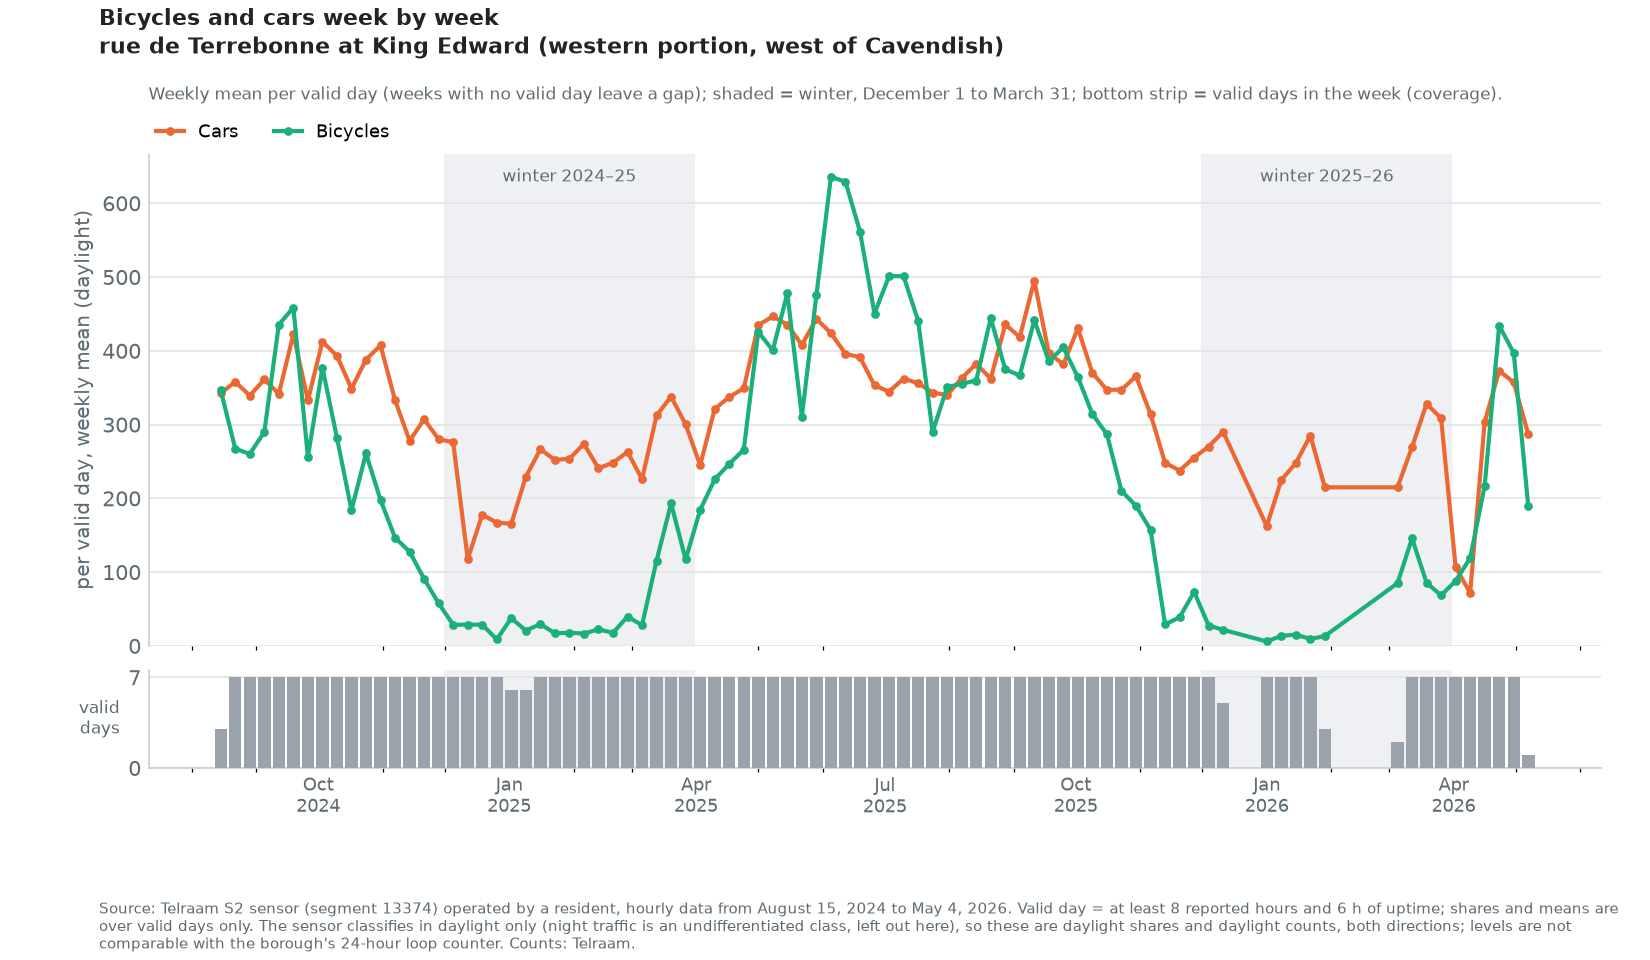
\includegraphics[width=0.9\textwidth]{../figures/mode-shares/dec1/overview_west.png}\\{\scriptsize Weekly mean per valid day, daylight. The two lines cross in late spring and part in October; the shaded winters show bicycles at a tenth or less of the summer level while cars fall by about a third.}\end{frame}
\begin{frame}{King Edward, non-winter 2025: who used the street}\centering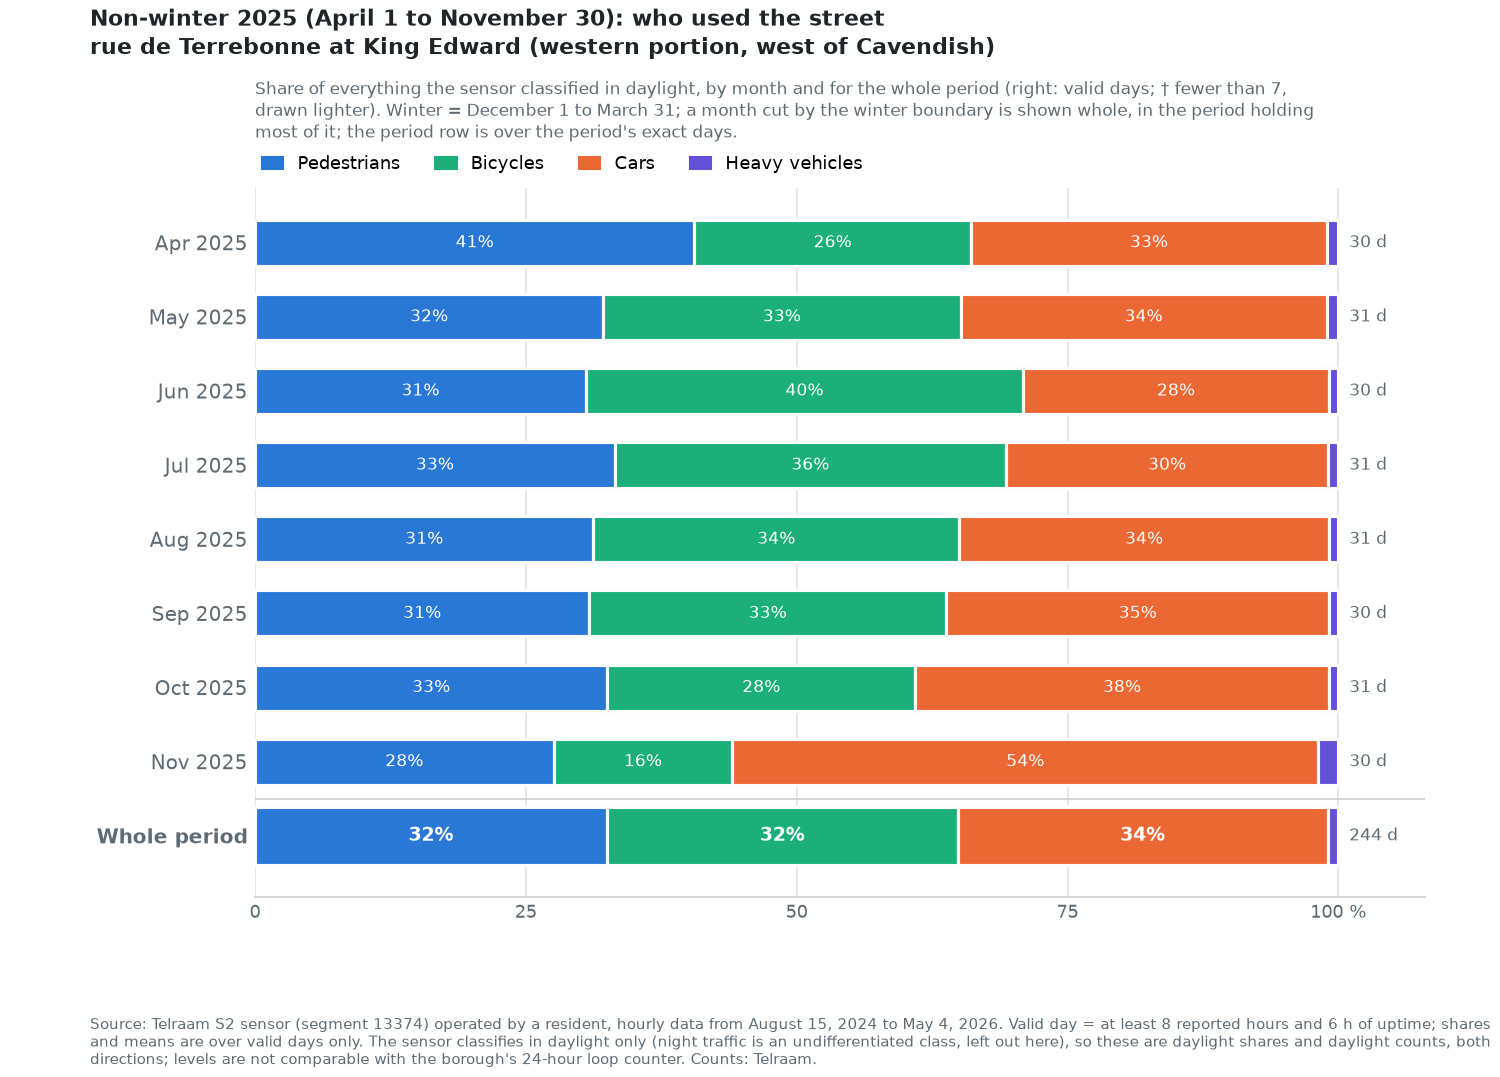
\includegraphics[width=0.8\textwidth]{../figures/mode-shares/dec1/shares_west_non-winter-2025.png}\\{\scriptsize Three roughly equal thirds from May to September; the car share rises in April, October and November.}\end{frame}
\begin{frame}{King Edward, non-winter 2025: daily counts by mode}\centering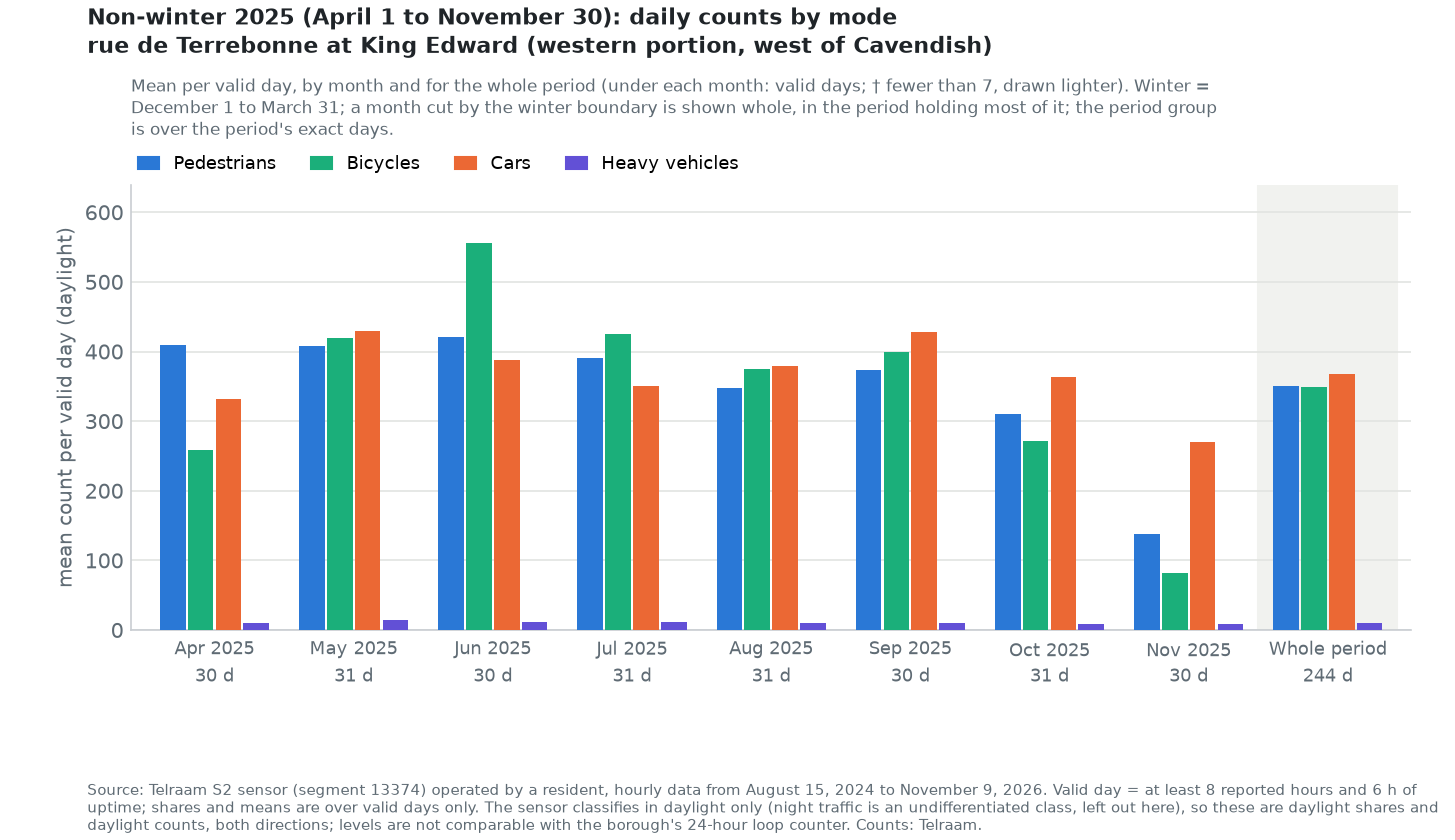
\includegraphics[width=0.86\textwidth]{../figures/mode-shares/dec1/counts_west_non-winter-2025.png}\end{frame}
\begin{frame}{King Edward, winter 2024--25: who used the street}\centering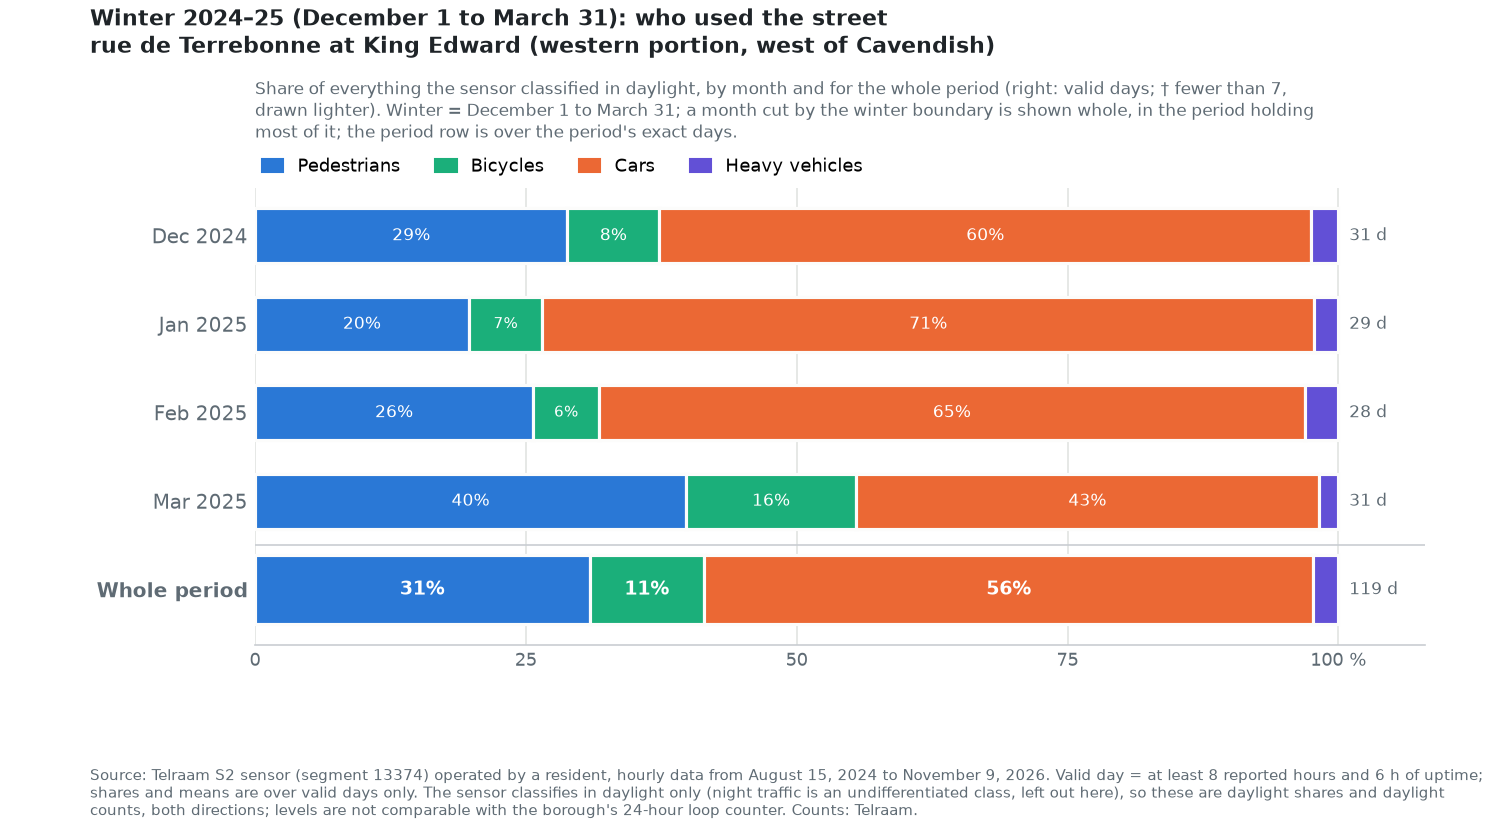
\includegraphics[width=0.8\textwidth]{../figures/mode-shares/dec1/shares_west_winter-2024-25.png}\end{frame}
\begin{frame}{King Edward, winter 2025--26: who used the street}\centering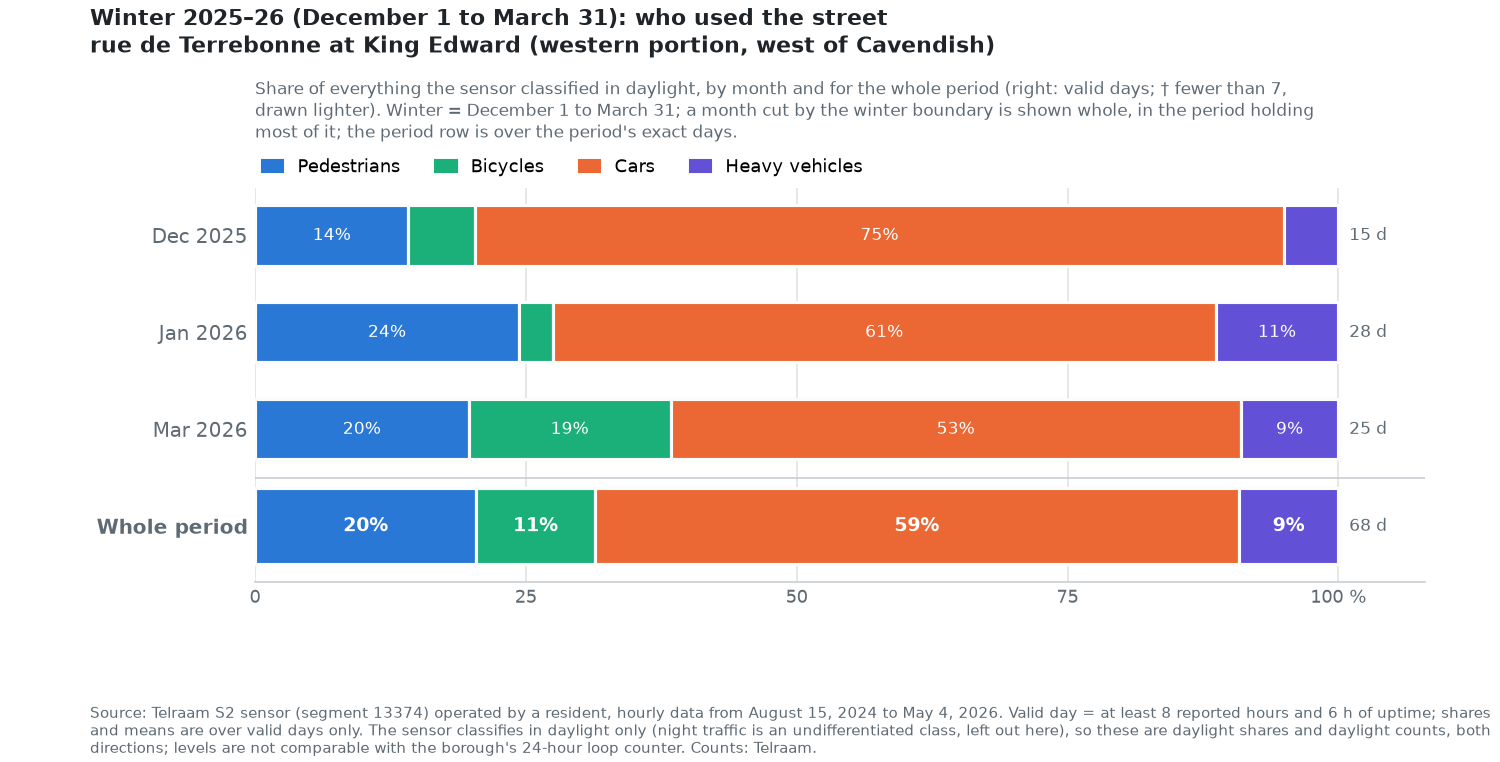
\includegraphics[width=0.8\textwidth]{../figures/mode-shares/dec1/shares_west_winter-2025-26.png}\\{\scriptsize 83 valid days: December has 15 and February none (outages). Heavy vehicles rose from about 10 a day to 35 a day this winter (44 a day in January); the cause is not examined here.}\end{frame}
\begin{frame}{King Edward, winter 2025--26: daily counts by mode}\centering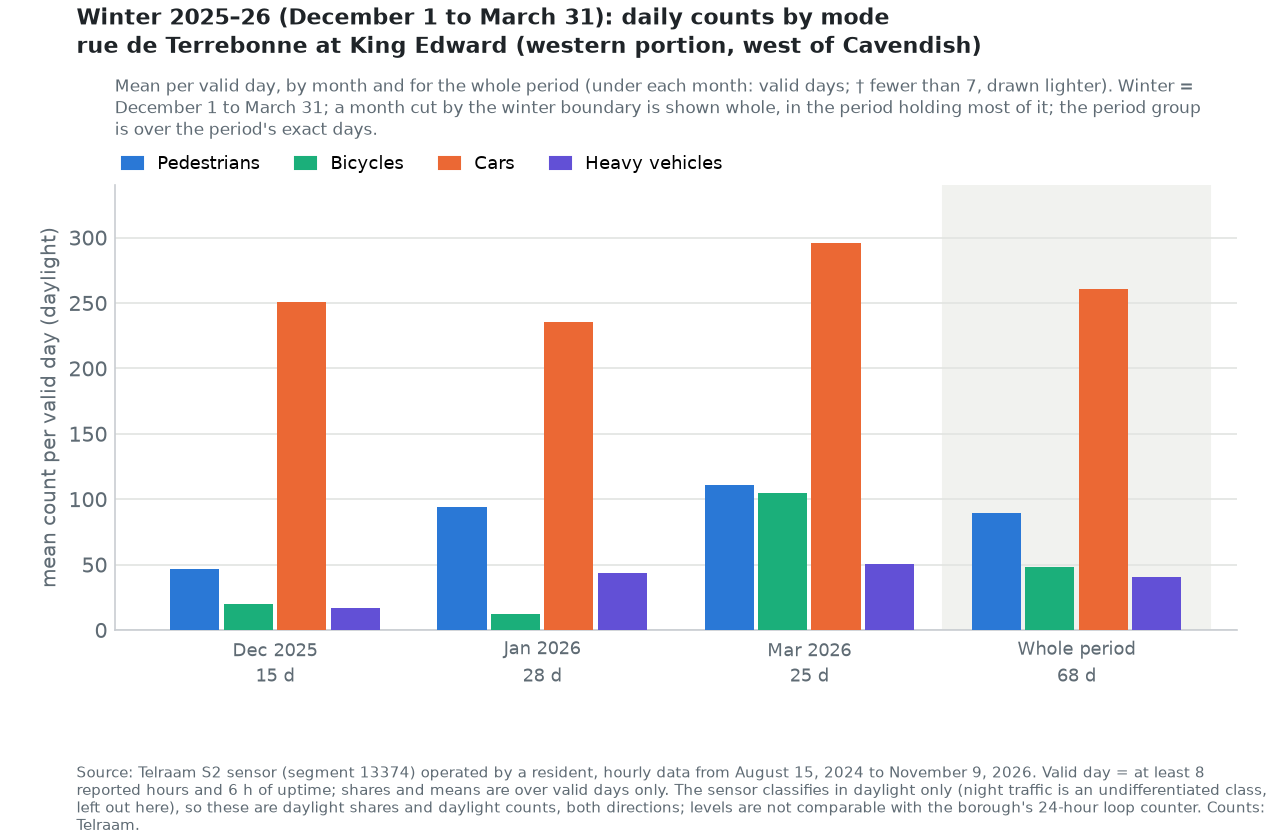
\includegraphics[width=0.86\textwidth]{../figures/mode-shares/dec1/counts_west_winter-2025-26.png}\end{frame}
\begin{frame}{Is cycling increasing at King Edward? Same months, year over year}\centering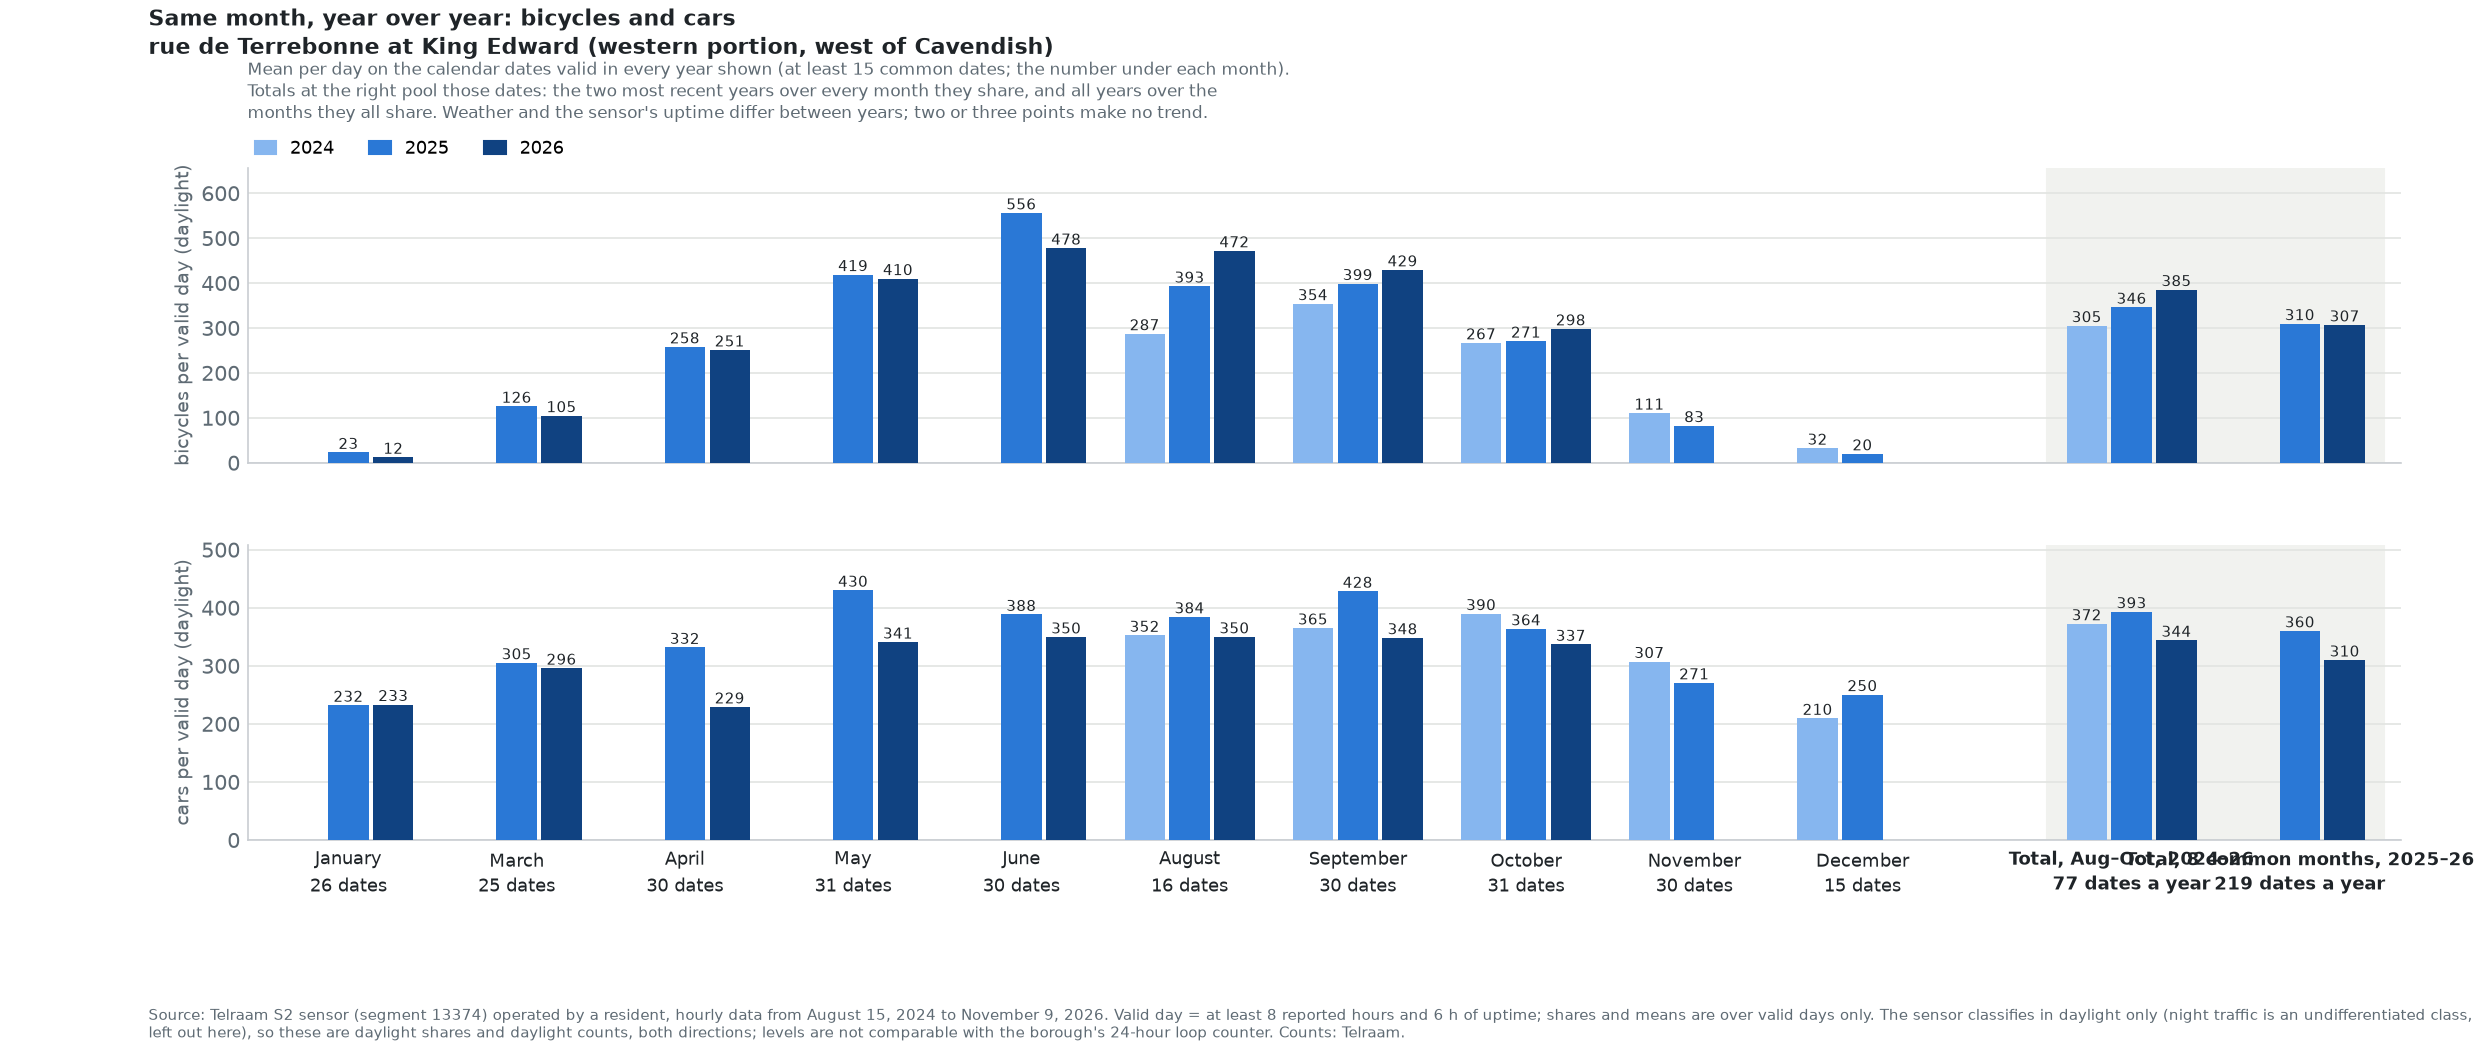
\includegraphics[width=0.72\textwidth]{../figures/mode-shares/dec1/yoy_west.png}\\{\scriptsize Mean per day on the dates valid in every year shown. August 2024 → 2025 → 2026: 287, 393, 472 bicycles a day; September 354, 399, 429; October 267, 271, 298. Totals on the same dates: August–October 305, 346, 385 a day (2024, 2025, 2026); over the eight months 2025 and 2026 share, 310 and 307, level, while cars fell from 360 to 310. The increase is a late-season one; spring 2026 was level with 2025 and June below. July 2026 (ten reported days, outage) is not shown.}\end{frame}
\section{Draper, the eastern portion}
\begin{frame}{Draper: bicycles and cars week by week}\centering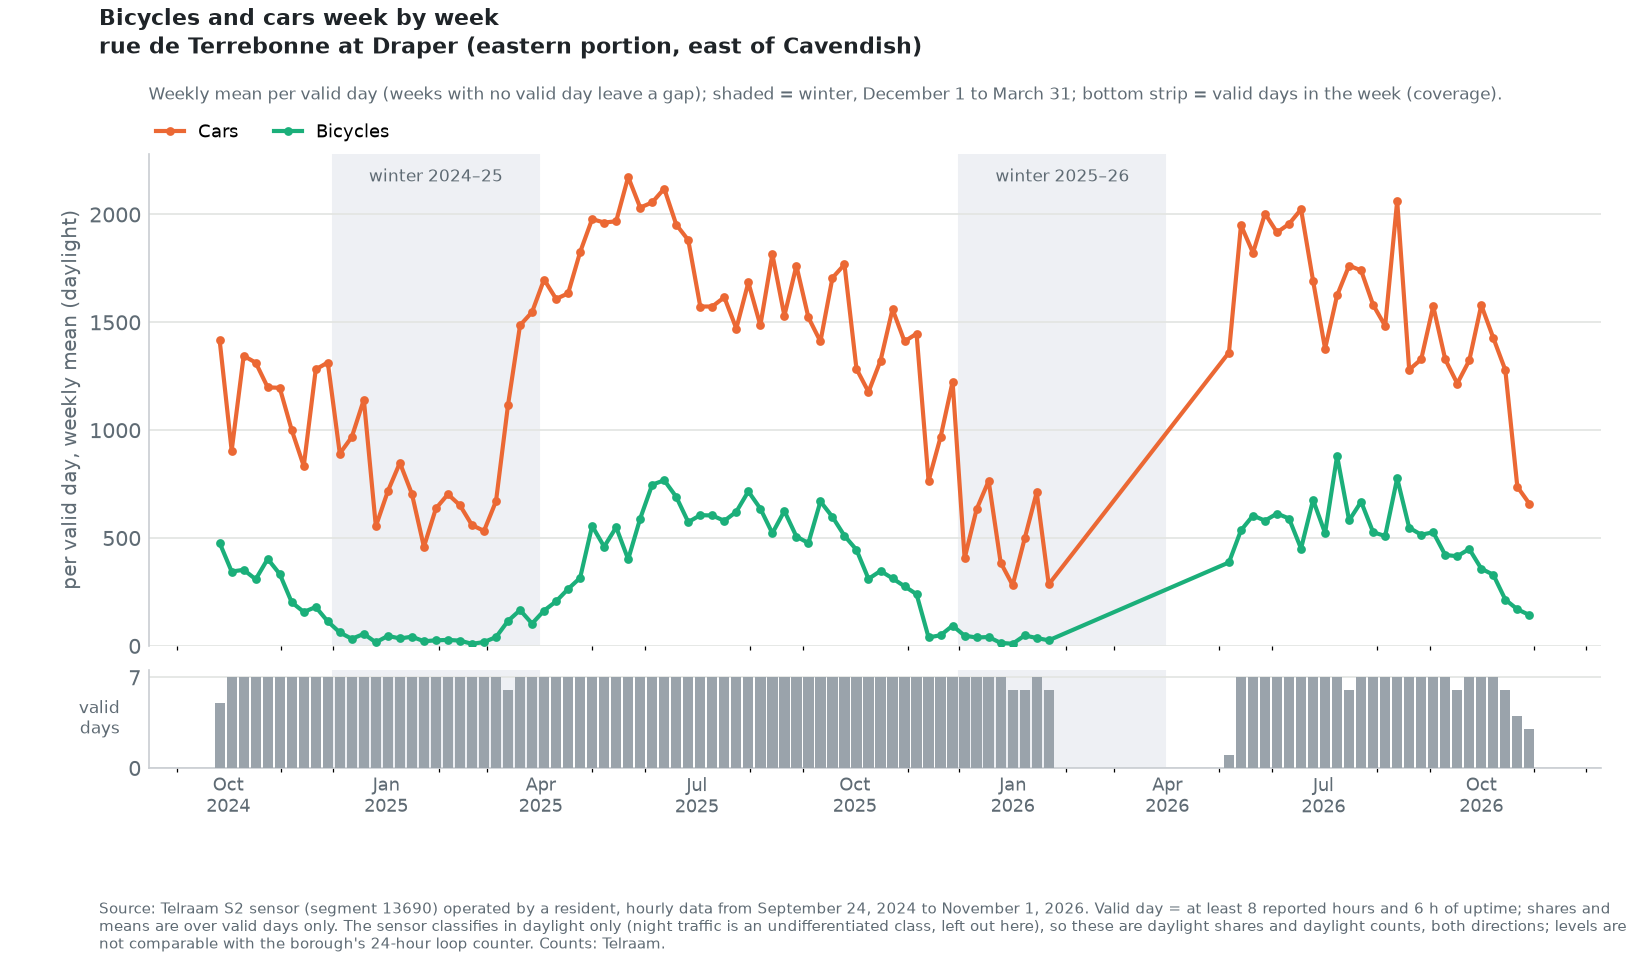
\includegraphics[width=0.9\textwidth]{../figures/mode-shares/dec1/overview_east.png}\\{\scriptsize Car volumes four times those at King Edward (the street is one-way eastbound here and carries through traffic to Girouard); bicycles at about three in ten cars in summer, one in fifteen in winter. The sensor stopped on January 24, 2026.}\end{frame}
\begin{frame}{Draper, non-winter 2025: who used the street}\centering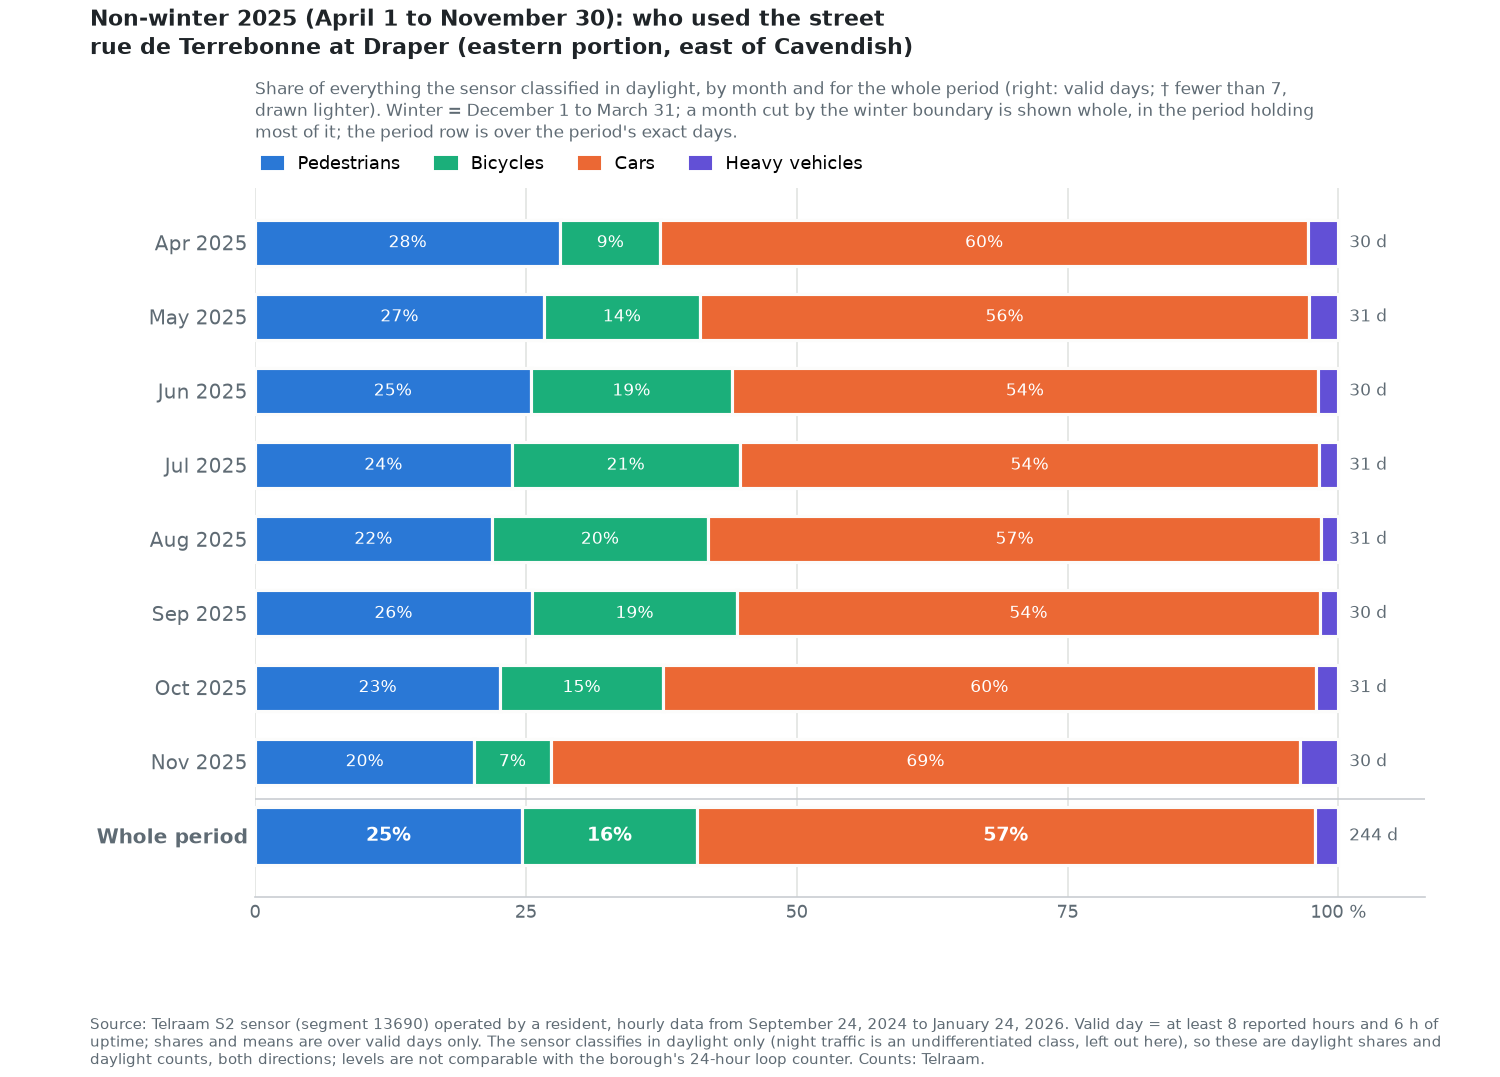
\includegraphics[width=0.8\textwidth]{../figures/mode-shares/dec1/shares_east_non-winter-2025.png}\end{frame}
\begin{frame}{Draper, winter 2024--25: who used the street}\centering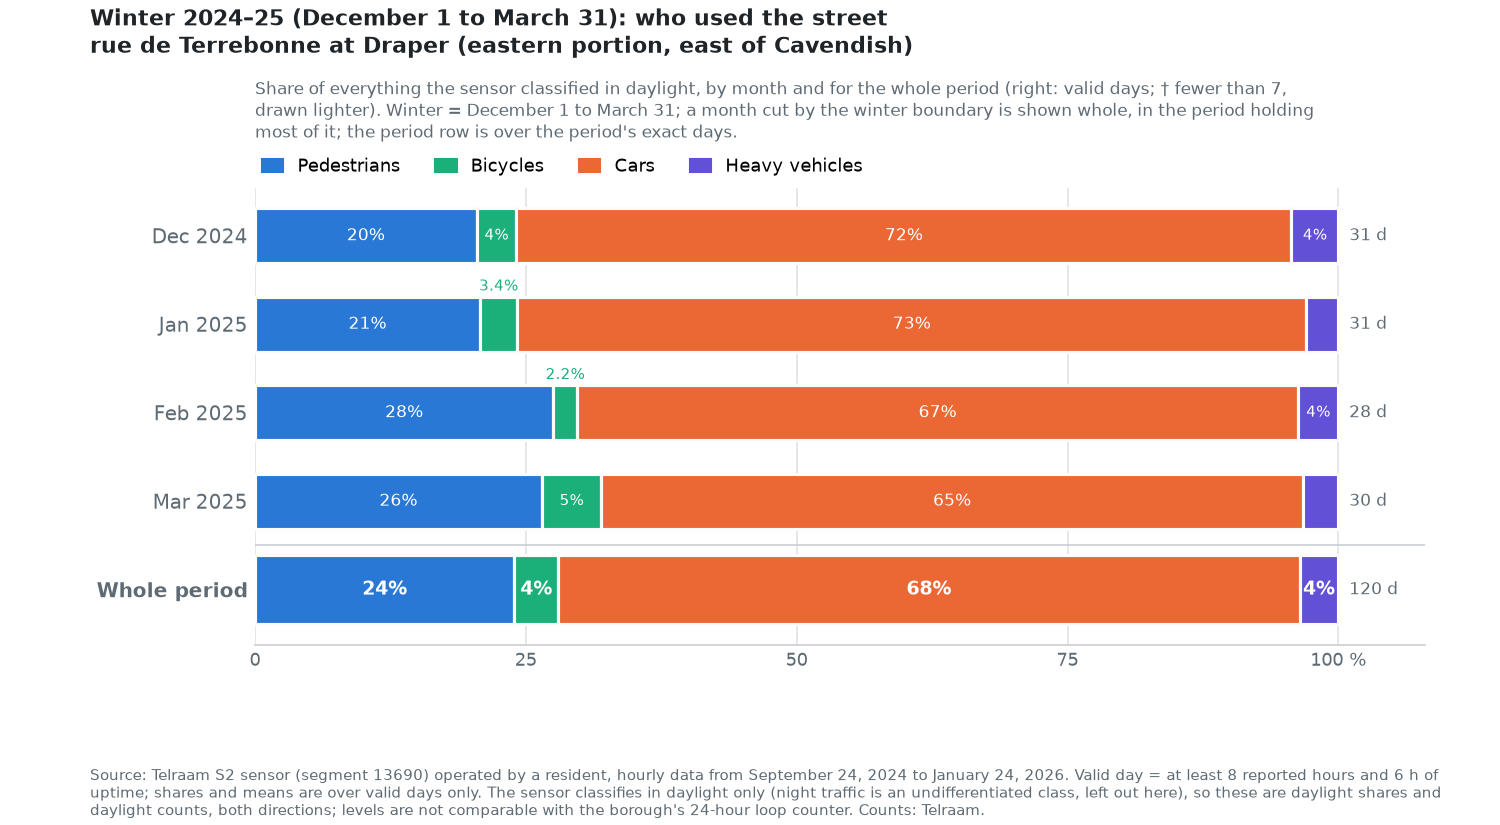
\includegraphics[width=0.8\textwidth]{../figures/mode-shares/dec1/shares_east_winter-2024-25.png}\end{frame}
\section{Kensington, the borough\textquoteright{}s loop counter}
\begin{frame}{Kensington loop: bicycles and motor vehicles week by week (24 h)}\centering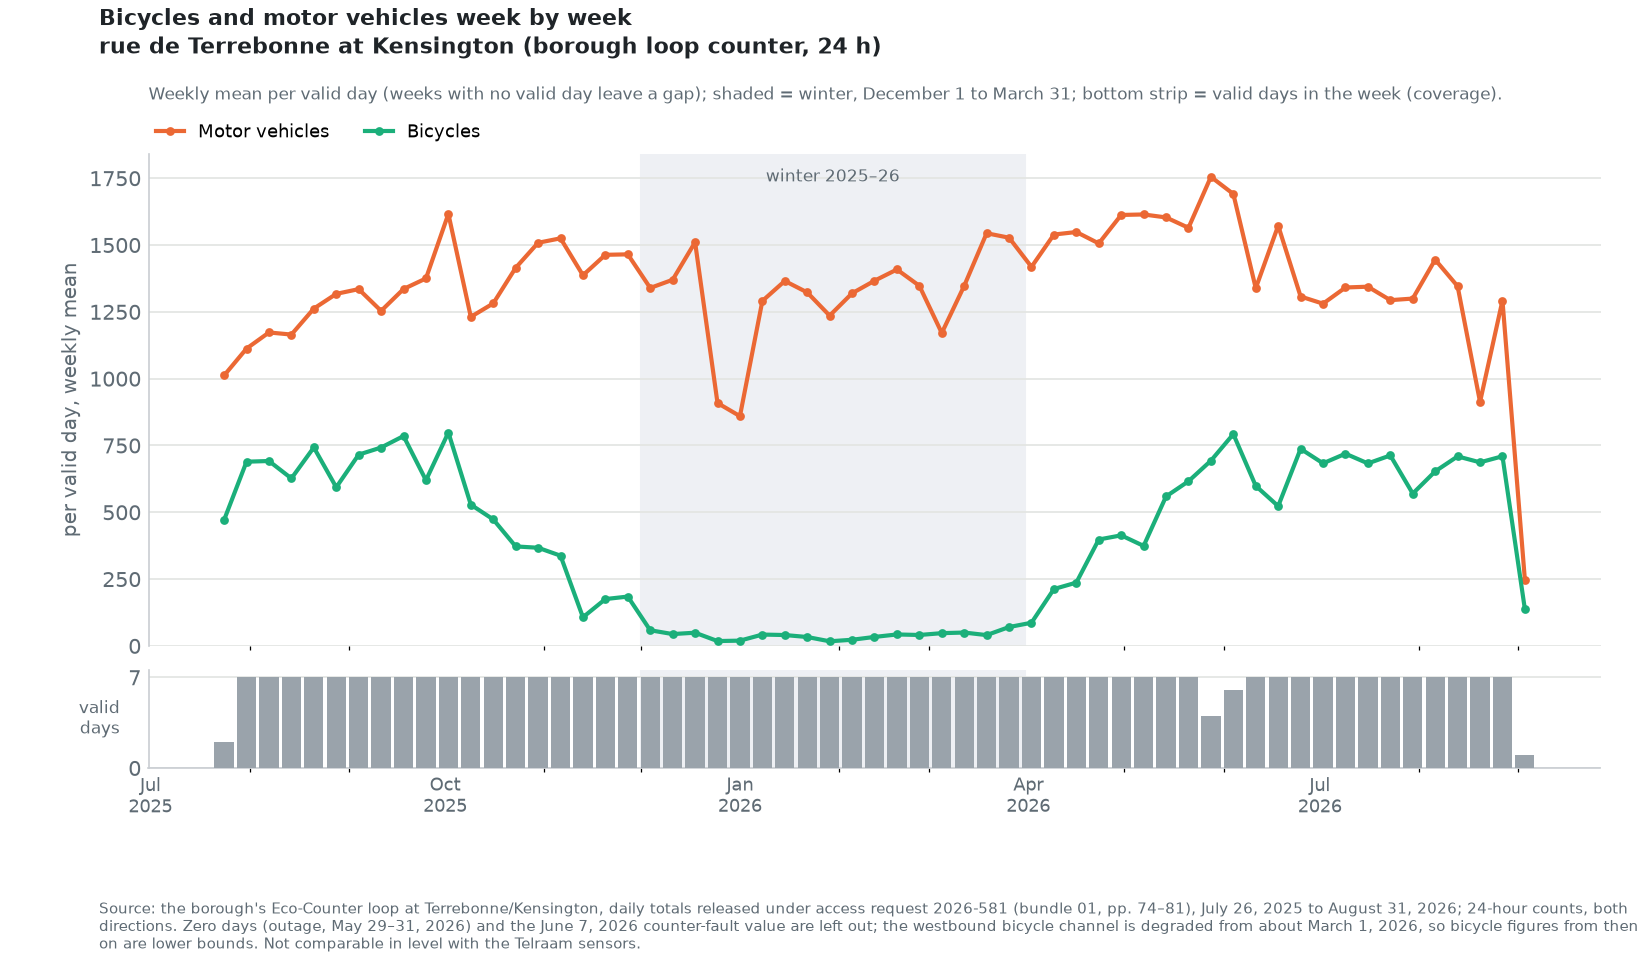
\includegraphics[width=0.9\textwidth]{../figures/mode-shares/dec1/overview_kensington.png}\\{\scriptsize The official record, 24 hours, both directions. Bicycle figures from March 2026 are lower bounds (westbound channel degraded).}\end{frame}
\begin{frame}{Kensington loop, non-winter 2025: what the loop counted}\centering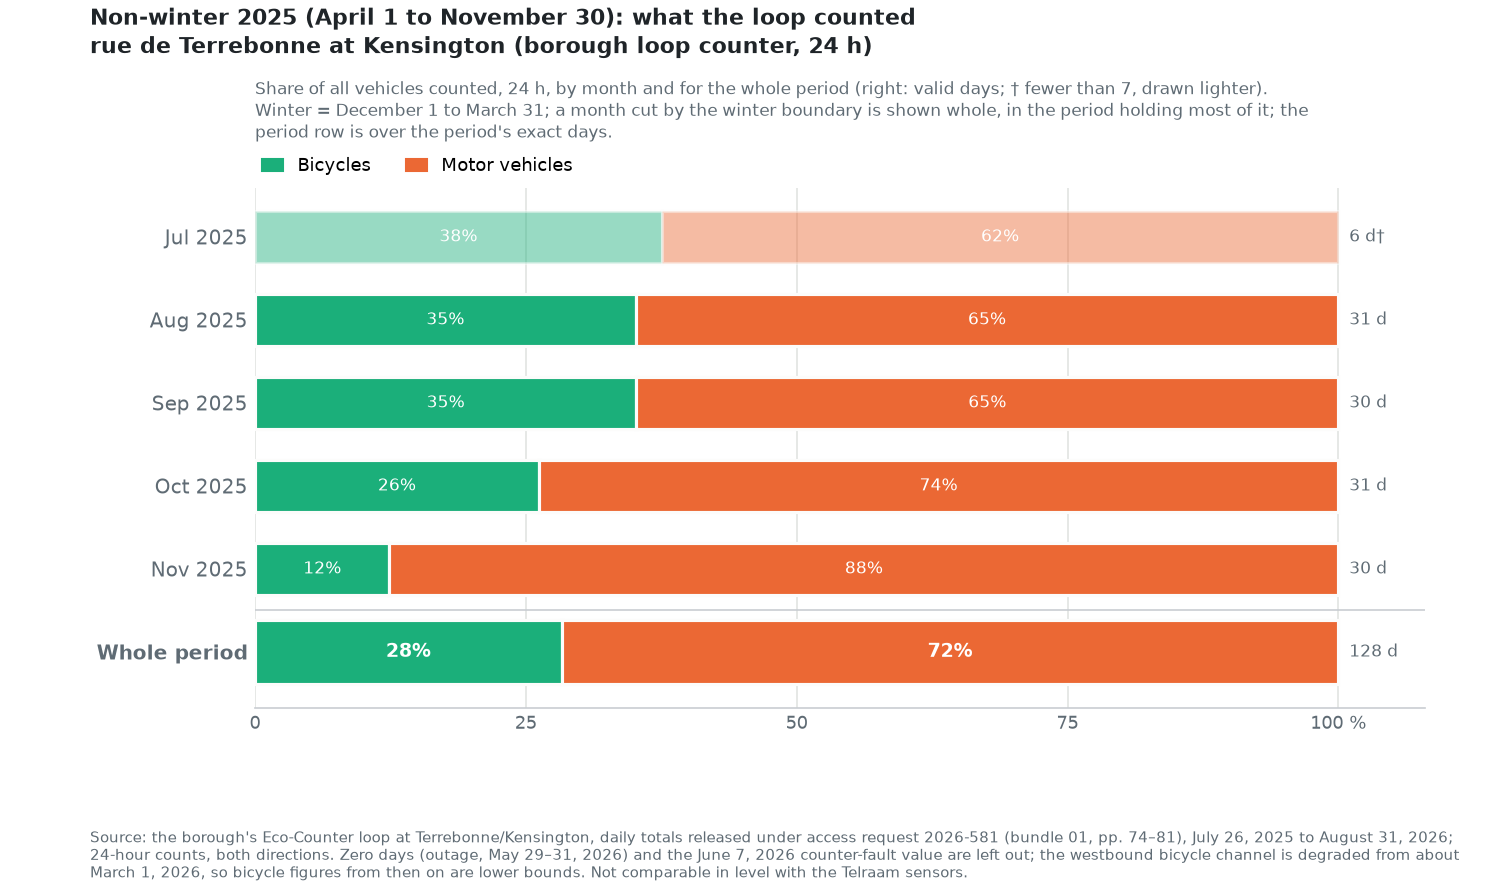
\includegraphics[width=0.8\textwidth]{../figures/mode-shares/dec1/shares_kensington_non-winter-2025.png}\\{\scriptsize Two modes only (the loop does not see pedestrians). Bicycles three in ten of all vehicles over 24 hours, July 26 to November 15, 2025.}\end{frame}
\begin{frame}{Kensington loop, winter 2025--26: what the loop counted}\centering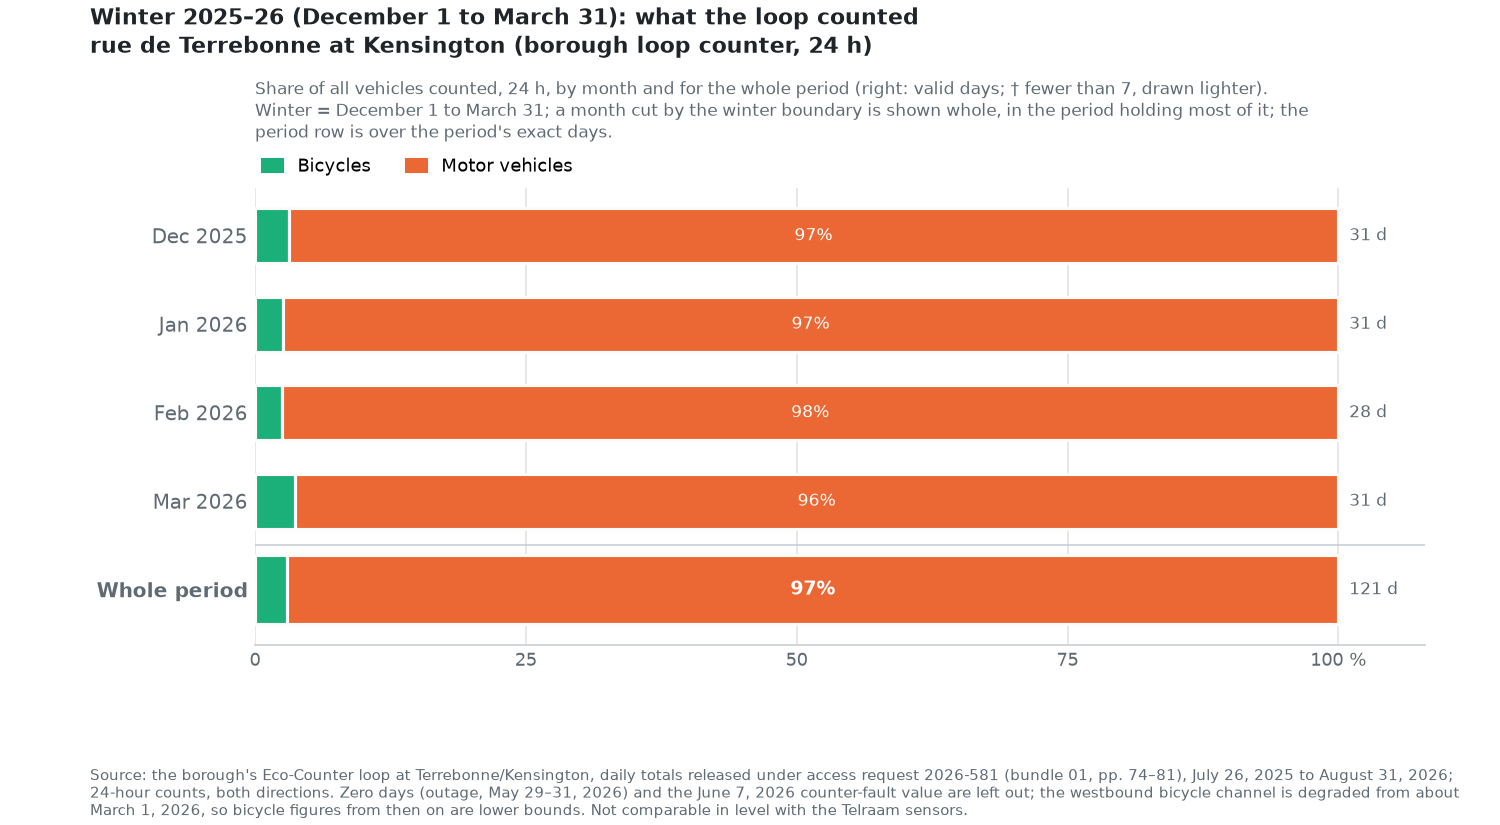
\includegraphics[width=0.8\textwidth]{../figures/mode-shares/dec1/shares_kensington_winter-2025-26.png}\end{frame}
\section{Summary tables}
\begin{frame}{Every counter and period, winter = December 1 to March 31}\centering{\scriptsize
\resizebox{\textwidth}{!}{\begin{tabular}{llrrrrrr}\toprule
Counter & Period & Valid days & Pedestrians & Bicycles & Cars & Heavy & Bicycles per 100 cars\\\midrule
King Edward (western portion) & Non-winter 2024 (08-15 to 11-30) & 107 & 35\,\% & 26\,\% & 37\,\% & 2\,\% & 71\\
King Edward (western portion) & Non-winter 2025 (04-01 to 11-30) & 244 & 32\,\% & 32\,\% & 34\,\% & 1\,\% & 95\\
King Edward (western portion) & Non-winter 2026 (04-01 to 11-09) & 194 & 29\,\% & 37\,\% & 31\,\% & 4\,\% & 119\\
King Edward (western portion) & Winter 2024–25 (12-01 to 03-31) & 119 & 31\,\% & 11\,\% & 56\,\% & 2\,\% & 19\\
King Edward (western portion) & Winter 2025–26 (12-01 to 03-31) & 68 & 20\,\% & 11\,\% & 60\,\% & 9\,\% & 18\\
\addlinespace
Draper (eastern portion) & Non-winter 2024 (09-24 to 11-30) & 67 & 28\,\% & 14\,\% & 56\,\% & 3\,\% & 24\\
Draper (eastern portion) & Non-winter 2025 (04-01 to 11-30) & 244 & 25\,\% & 16\,\% & 57\,\% & 2\,\% & 28\\
Draper (eastern portion) & Non-winter 2026 (04-01 to 11-01) & 166 & 23\,\% & 19\,\% & 57\,\% & 2\,\% & 33\\
Draper (eastern portion) & Winter 2024–25 (12-01 to 03-31) & 120 & 24\,\% & 4\,\% & 68\,\% & 4\,\% & 6\\
Draper (eastern portion) & Winter 2025–26 (12-01 to 03-31) & 53 & 22\,\% & 5\,\% & 70\,\% & 4\,\% & 7\\
\addlinespace
Kensington loop (24 h) & Non-winter 2025 (07-26 to 11-30) & 128 & -- & 28\,\% & 72\,\%\textsuperscript{m} & -- & 40\\
Kensington loop (24 h) & Non-winter 2026 (04-01 to 08-31) & 149 & -- & 28\,\% & 72\,\%\textsuperscript{m} & -- & 40\\
Kensington loop (24 h) & Winter 2025–26 (12-01 to 03-31) & 121 & -- & 3\,\% & 97\,\%\textsuperscript{m} & -- & 3\\
\addlinespace
\bottomrule\end{tabular}}
\\[4pt] Shares of everything classified in daylight (Telraam) or of all vehicles counted over 24 h (loop; \textsuperscript{m} = motor vehicles). Periods with fewer than 20 valid days omitted. Non-winter periods are cut by the record\textquoteright{}s first and last days.}\end{frame}
\begin{frame}{The same with winter = November 16 to March 31}\centering{\scriptsize
\resizebox{\textwidth}{!}{\begin{tabular}{llrrrrrr}\toprule
Counter & Period & Valid days & Pedestrians & Bicycles & Cars & Heavy & Bicycles per 100 cars\\\midrule
King Edward (western portion) & Non-winter 2024 (08-15 to 11-15) & 92 & 35\,\% & 28\,\% & 36\,\% & 2\,\% & 76\\
King Edward (western portion) & Non-winter 2025 (04-01 to 11-15) & 229 & 33\,\% & 33\,\% & 34\,\% & 1\,\% & 98\\
King Edward (western portion) & Non-winter 2026 (04-01 to 11-09) & 194 & 29\,\% & 37\,\% & 31\,\% & 4\,\% & 119\\
King Edward (western portion) & Winter 2024–25 (11-16 to 03-31) & 134 & 32\,\% & 11\,\% & 55\,\% & 2\,\% & 20\\
King Edward (western portion) & Winter 2025–26 (11-16 to 03-31) & 83 & 21\,\% & 11\,\% & 60\,\% & 8\,\% & 19\\
\addlinespace
Draper (eastern portion) & Non-winter 2024 (09-24 to 11-15) & 52 & 28\,\% & 15\,\% & 54\,\% & 3\,\% & 28\\
Draper (eastern portion) & Non-winter 2025 (04-01 to 11-15) & 229 & 25\,\% & 16\,\% & 56\,\% & 2\,\% & 29\\
Draper (eastern portion) & Non-winter 2026 (04-01 to 11-01) & 166 & 23\,\% & 19\,\% & 57\,\% & 2\,\% & 33\\
Draper (eastern portion) & Winter 2024–25 (11-16 to 03-31) & 135 & 24\,\% & 5\,\% & 67\,\% & 4\,\% & 7\\
Draper (eastern portion) & Winter 2025–26 (11-16 to 03-31) & 68 & 20\,\% & 5\,\% & 71\,\% & 4\,\% & 6\\
\addlinespace
Kensington loop (24 h) & Non-winter 2025 (07-26 to 11-15) & 113 & -- & 30\,\% & 70\,\%\textsuperscript{m} & -- & 44\\
Kensington loop (24 h) & Non-winter 2026 (04-01 to 08-31) & 149 & -- & 28\,\% & 72\,\%\textsuperscript{m} & -- & 40\\
Kensington loop (24 h) & Winter 2025–26 (11-16 to 03-31) & 136 & -- & 4\,\% & 96\,\%\textsuperscript{m} & -- & 4\\
\addlinespace
\bottomrule\end{tabular}}
\\[4pt] The borough\textquoteright{}s proposed conversion window. The shares move by a point or two: the second half of November is a transition fortnight, not a winter one, at either end of the street.}\end{frame}
\begin{frame}{Cautions}\begin{itemize}
\item \textbf{Daylight only.} The Telraam shares exclude night traffic, which is mostly motor traffic. The loop counter\textquoteright{}s 24-hour ratio (about 44 bicycles per 100 motor vehicles outside winter at Kensington) is the comparable official figure; the Telraam sensors are the check and the history, not the record.
\item \textbf{Two ends, two streets.} West of Cavendish the street is one-way westbound with about 350 cars a day in daylight; east of it, one-way eastbound with about 1,500. A statement about « the western portion » does not transfer to the whole street.
\item \textbf{Classification.} Telraam\textquoteright{}s classes are the sensor\textquoteright{}s; the winter rise in « heavy vehicles » at King Edward may be snow equipment, classification drift, or both. The snow-day divergence between Telraam and the loop (Terrebonne-open-sources, 2026-winter-counts-user-frequency) is unresolved.
\item \textbf{The record ends May 4, 2026} at King Edward. Extending it needs a Telraam API token or a new dashboard export; the dashboard\textquoteright{}s recent months, with their outages, are not in these figures.
\item Code, tables, figures: \url{https://github.com/OpenMobilityData/Terrebonne-telraam}. Counts: Telraam (its terms of use; the exports are not republished) and the borough\textquoteright{}s release under access request 2026-581.
\end{itemize}\end{frame}
\appendix
\section{Appendix: the remaining figures}
\begin{frame}{Draper (eastern portion), non--winter 2024: daily counts by mode}\centering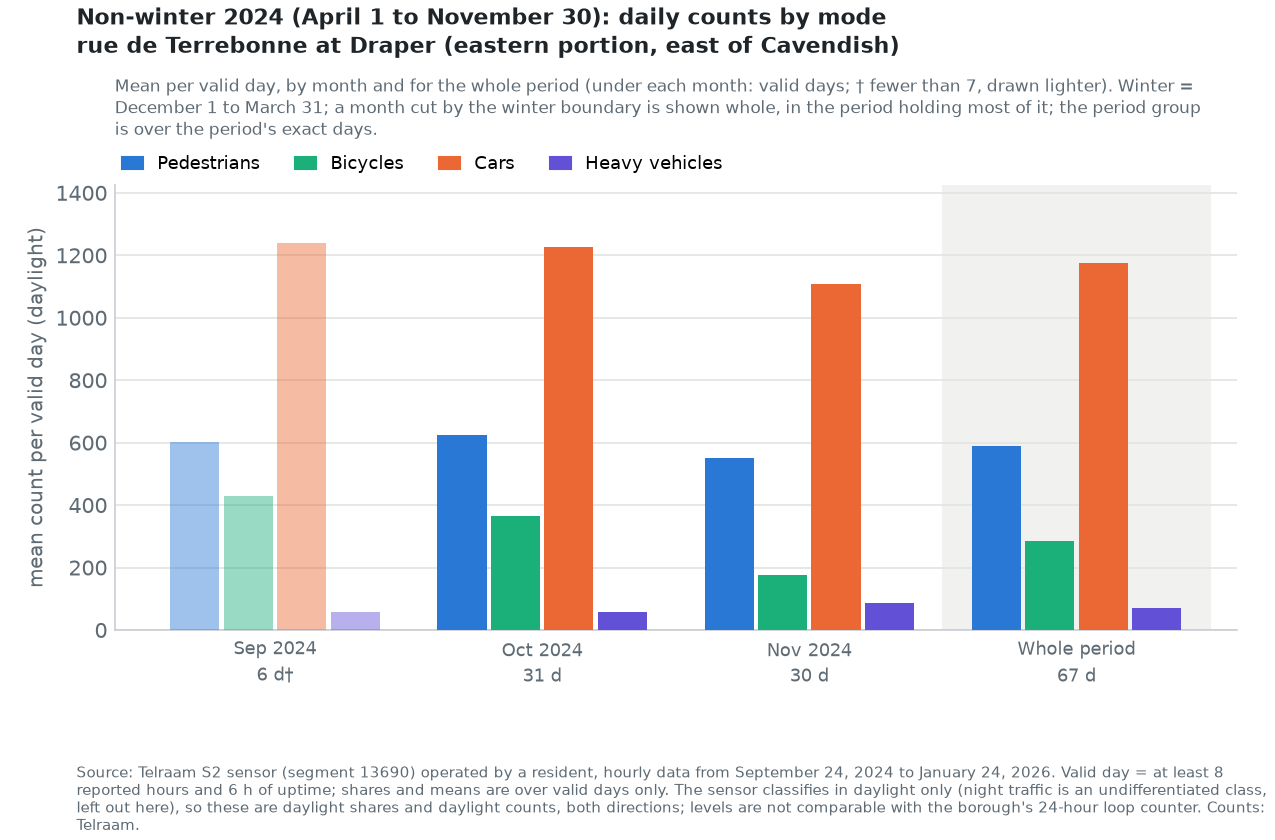
\includegraphics[width=0.86\textwidth]{../figures/mode-shares/dec1/counts_east_non-winter-2024.png}\end{frame}
\begin{frame}{Draper (eastern portion), non--winter 2025: daily counts by mode}\centering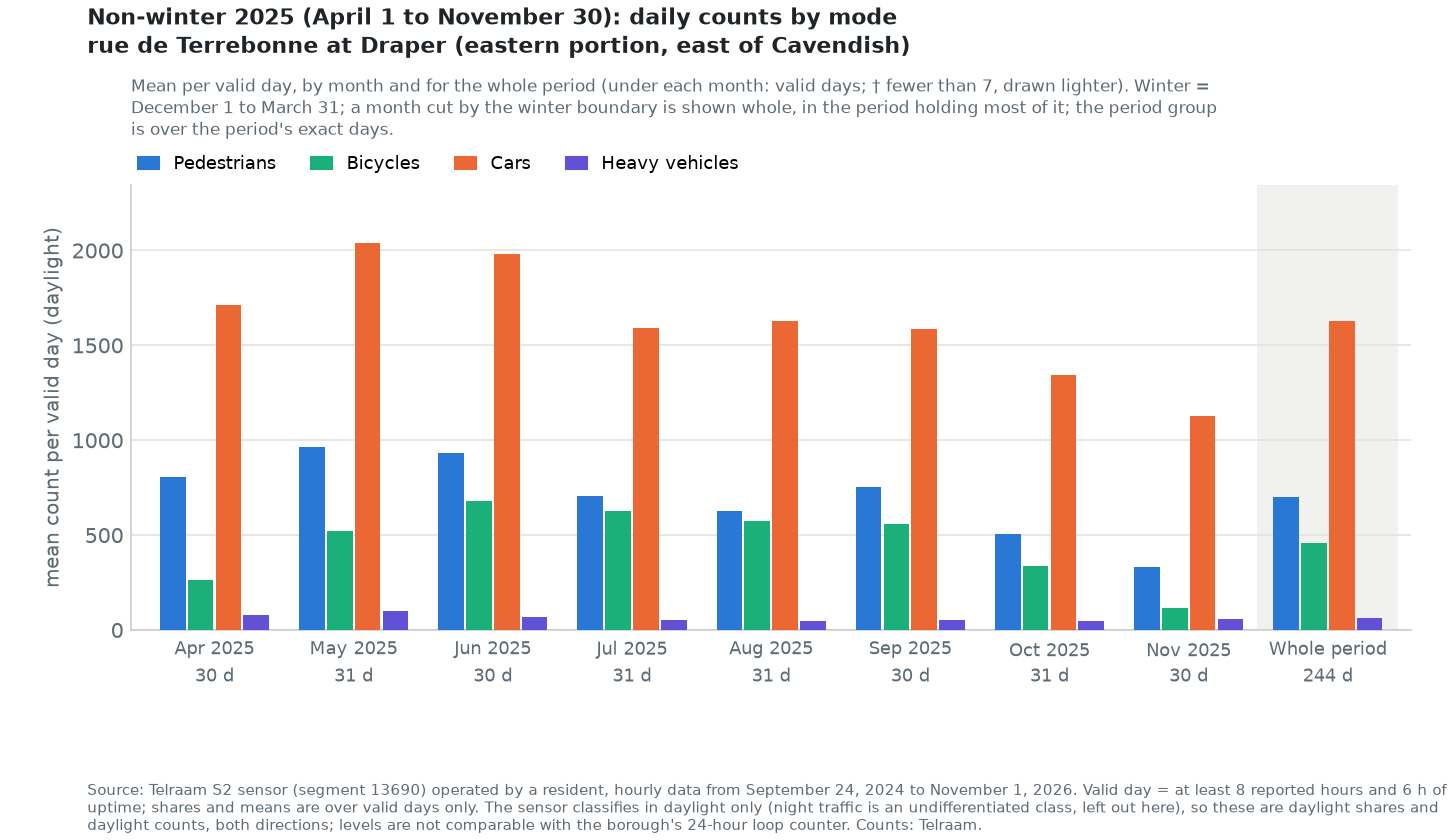
\includegraphics[width=0.86\textwidth]{../figures/mode-shares/dec1/counts_east_non-winter-2025.png}\end{frame}
\begin{frame}{Draper (eastern portion), non--winter 2026: daily counts by mode}\centering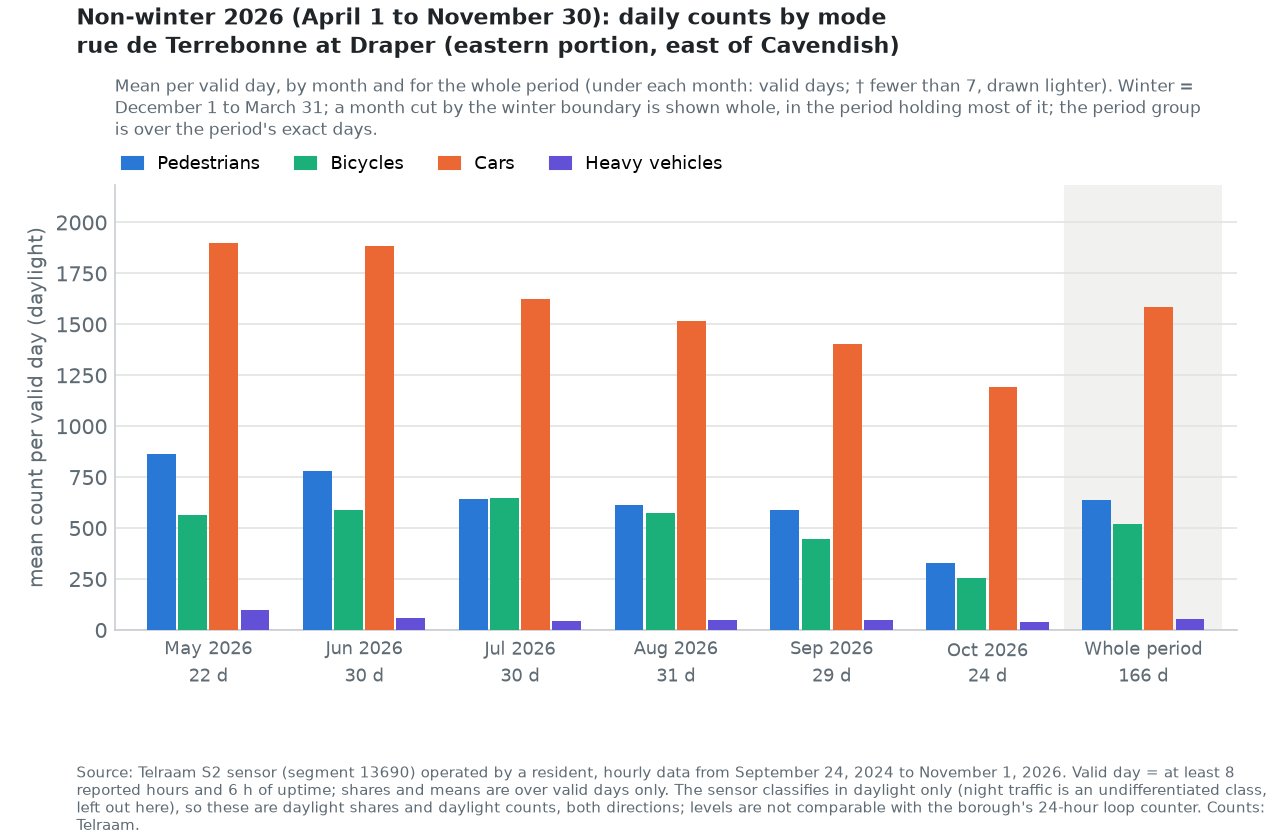
\includegraphics[width=0.86\textwidth]{../figures/mode-shares/dec1/counts_east_non-winter-2026.png}\end{frame}
\begin{frame}{Draper (eastern portion), winter 2024--25: daily counts by mode}\centering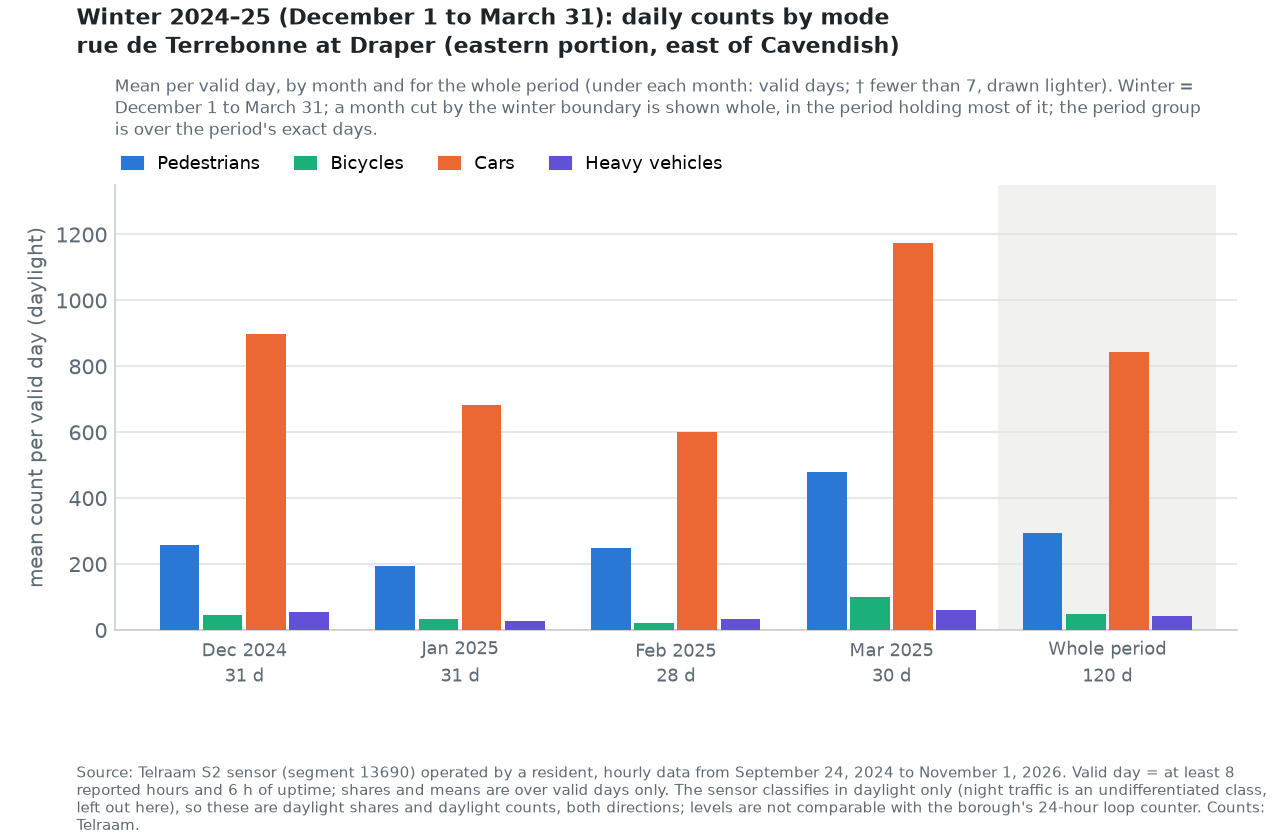
\includegraphics[width=0.86\textwidth]{../figures/mode-shares/dec1/counts_east_winter-2024-25.png}\end{frame}
\begin{frame}{Draper (eastern portion), winter 2025--26: daily counts by mode}\centering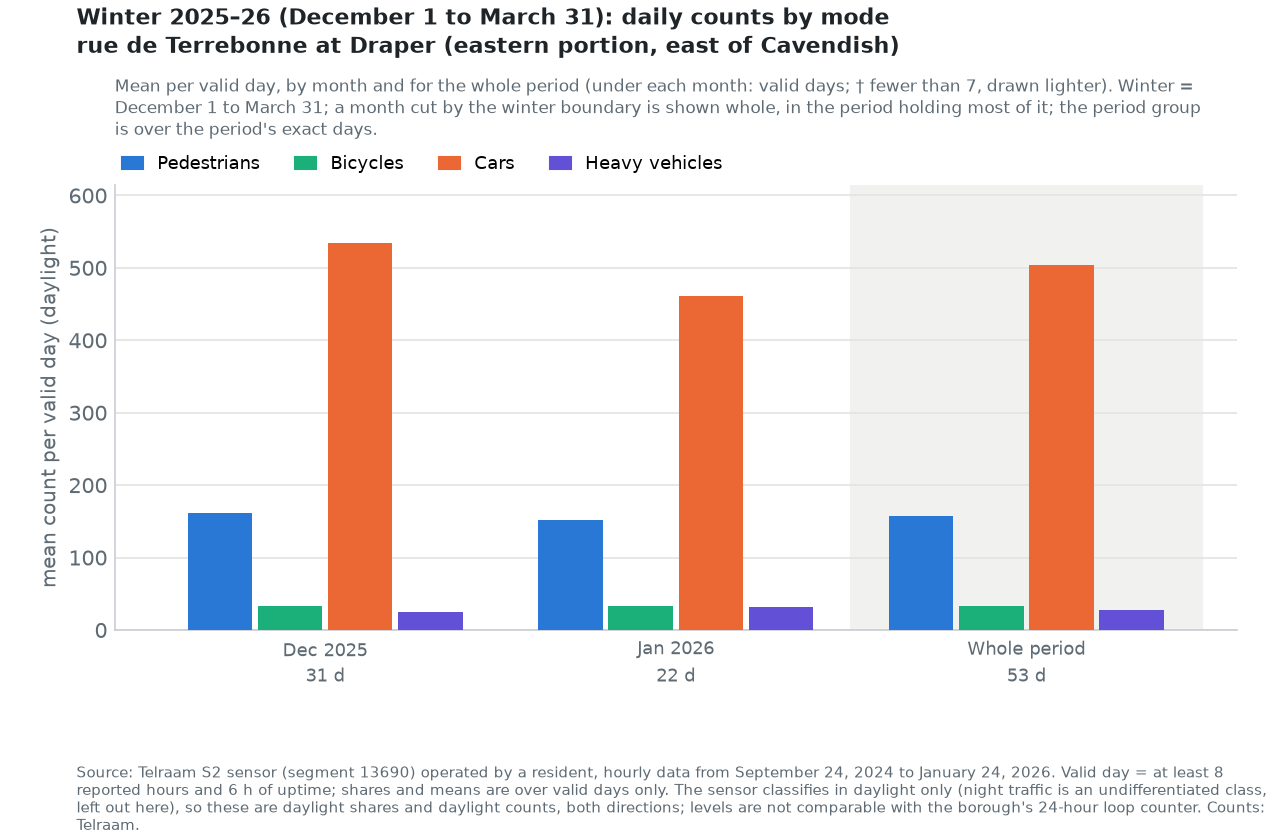
\includegraphics[width=0.86\textwidth]{../figures/mode-shares/dec1/counts_east_winter-2025-26.png}\end{frame}
\begin{frame}{Kensington loop (24 h), non--winter 2025: daily counts by mode}\centering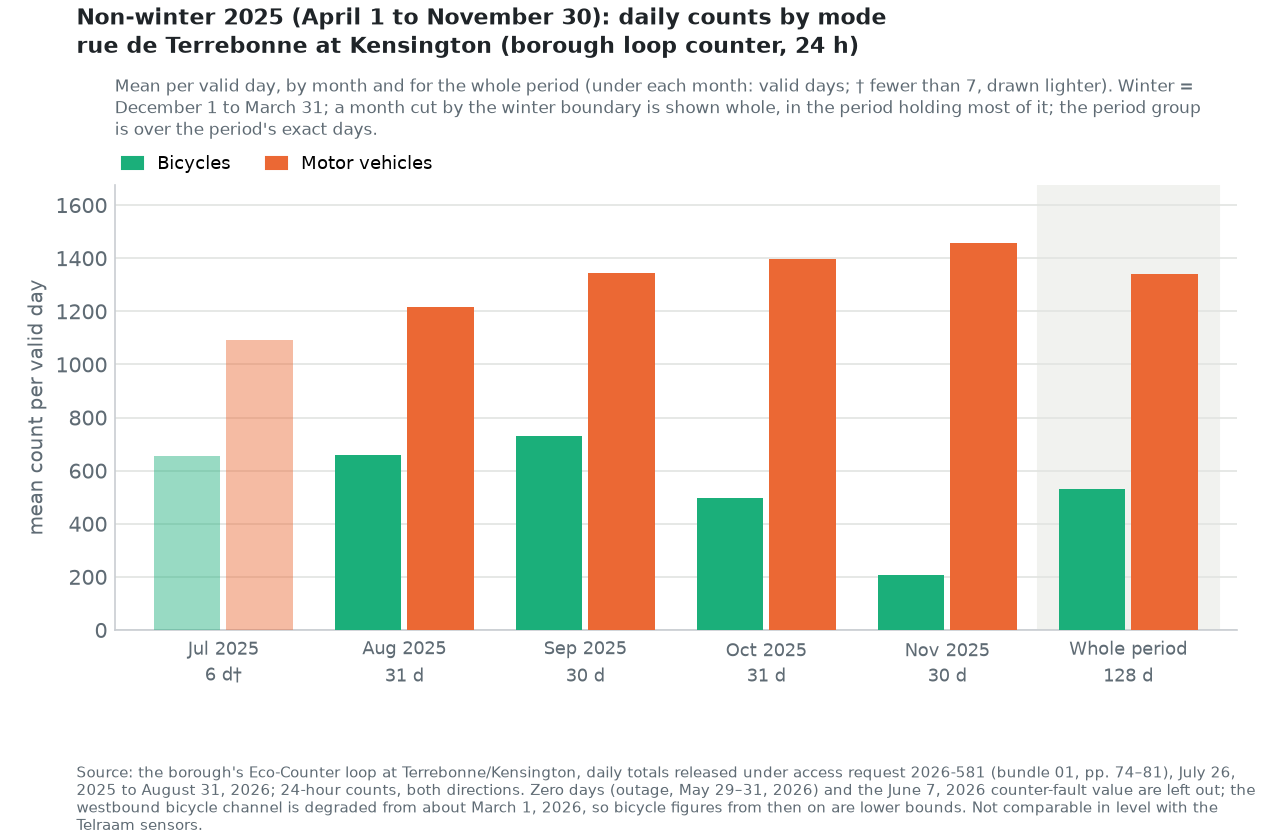
\includegraphics[width=0.86\textwidth]{../figures/mode-shares/dec1/counts_kensington_non-winter-2025.png}\end{frame}
\begin{frame}{Kensington loop (24 h), non--winter 2026: daily counts by mode}\centering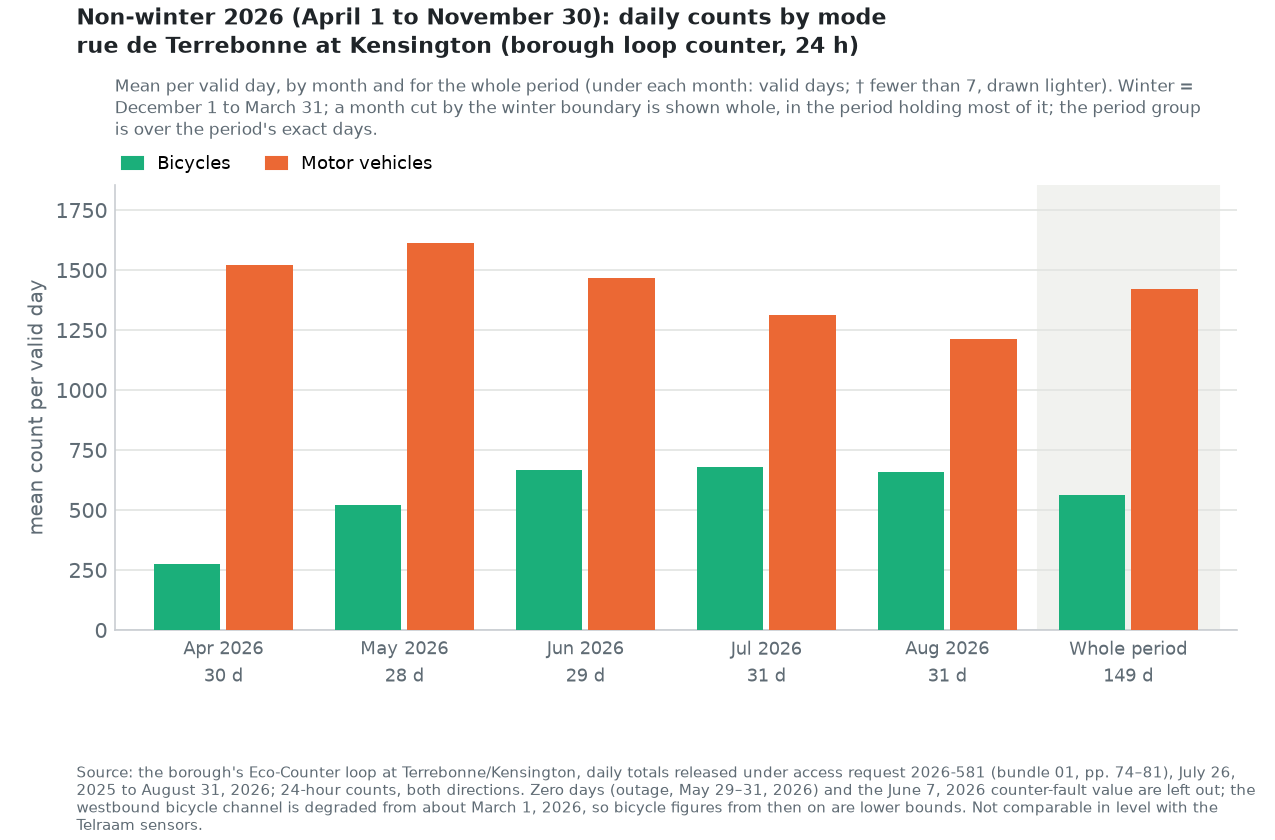
\includegraphics[width=0.86\textwidth]{../figures/mode-shares/dec1/counts_kensington_non-winter-2026.png}\end{frame}
\begin{frame}{Kensington loop (24 h), winter 2025--26: daily counts by mode}\centering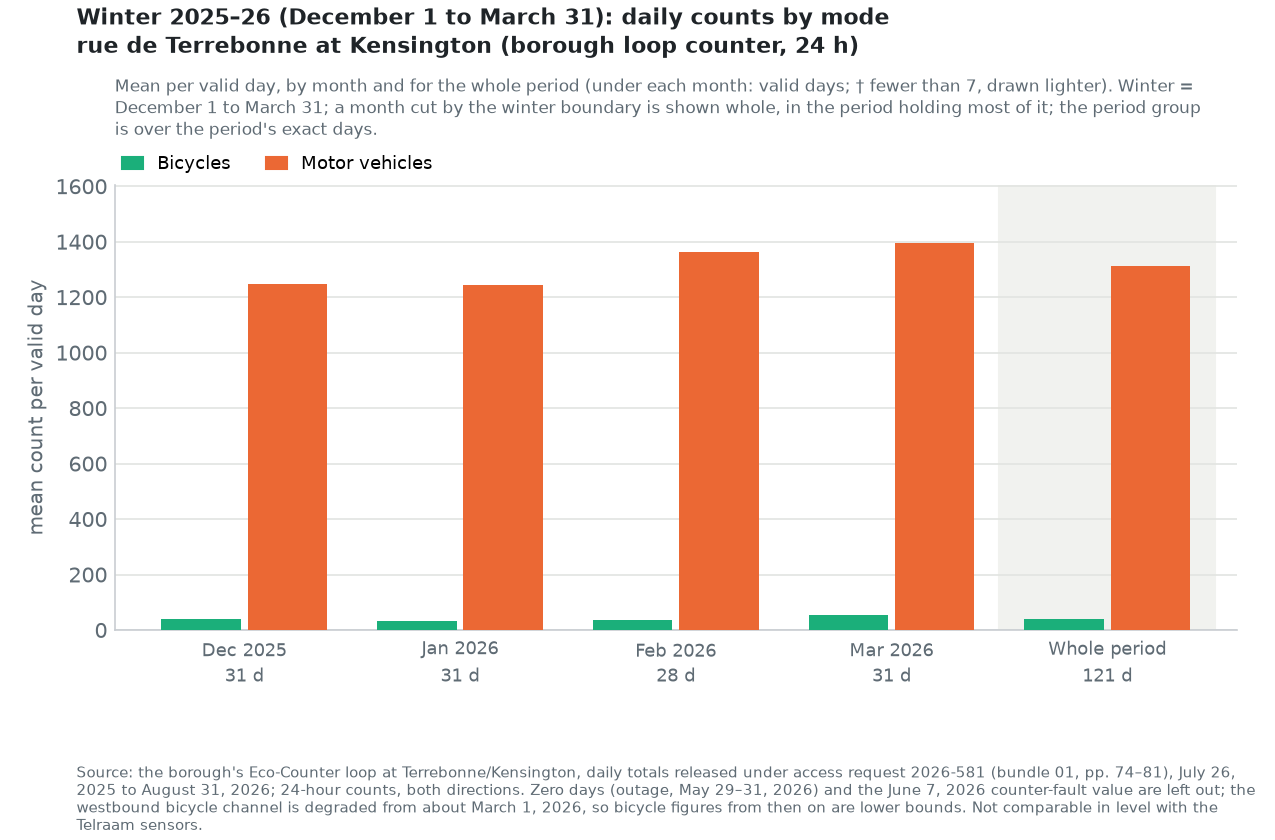
\includegraphics[width=0.86\textwidth]{../figures/mode-shares/dec1/counts_kensington_winter-2025-26.png}\end{frame}
\begin{frame}{King Edward (western portion), non--winter 2024: daily counts by mode}\centering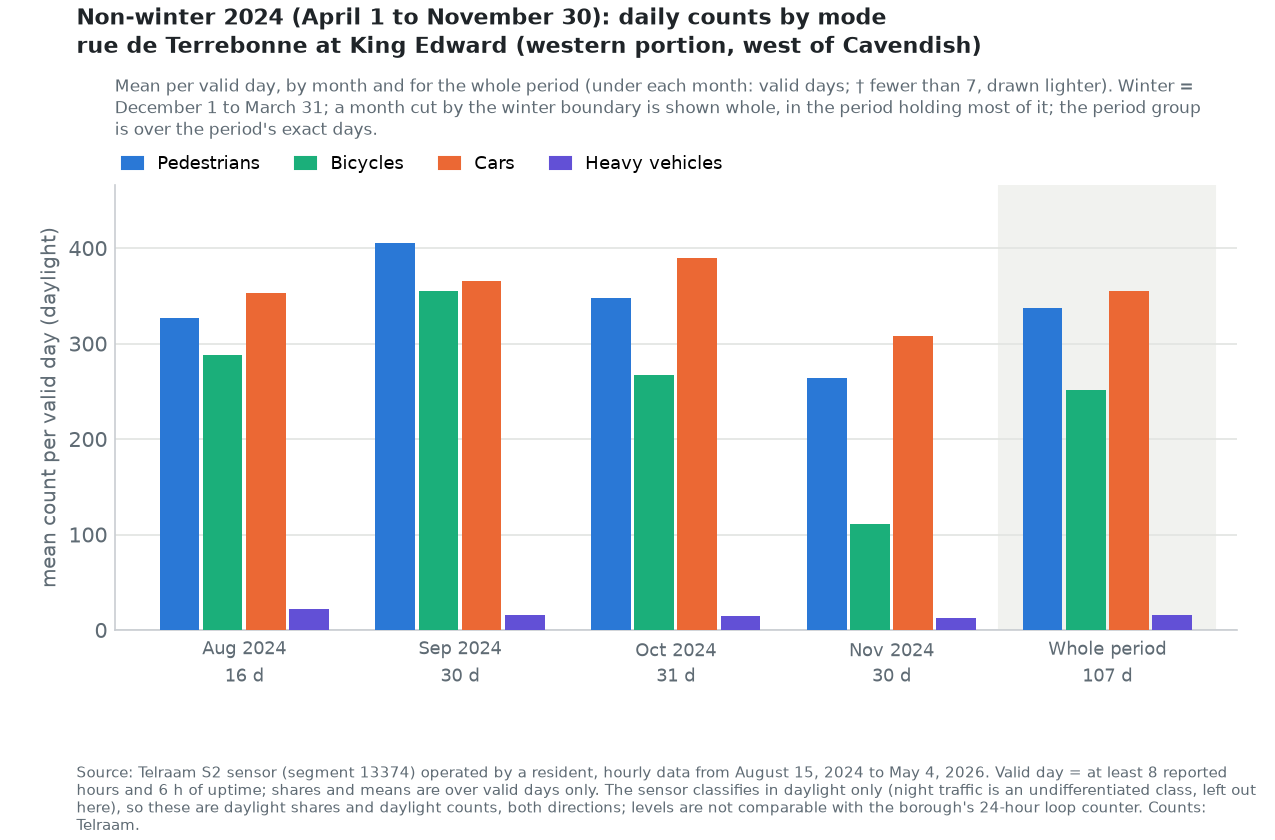
\includegraphics[width=0.86\textwidth]{../figures/mode-shares/dec1/counts_west_non-winter-2024.png}\end{frame}
\begin{frame}{King Edward (western portion), non--winter 2026: daily counts by mode}\centering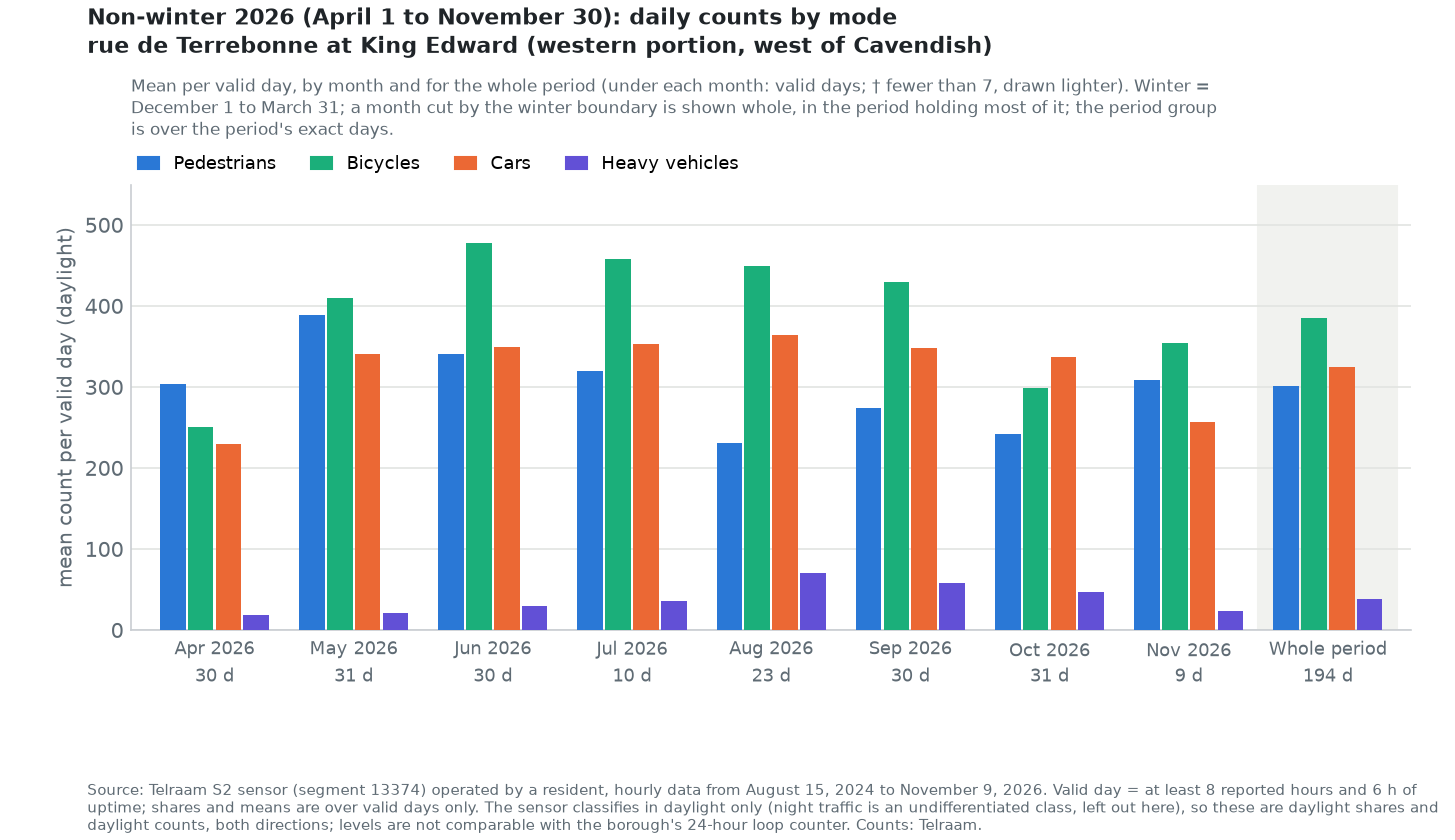
\includegraphics[width=0.86\textwidth]{../figures/mode-shares/dec1/counts_west_non-winter-2026.png}\end{frame}
\begin{frame}{King Edward (western portion), winter 2024--25: daily counts by mode}\centering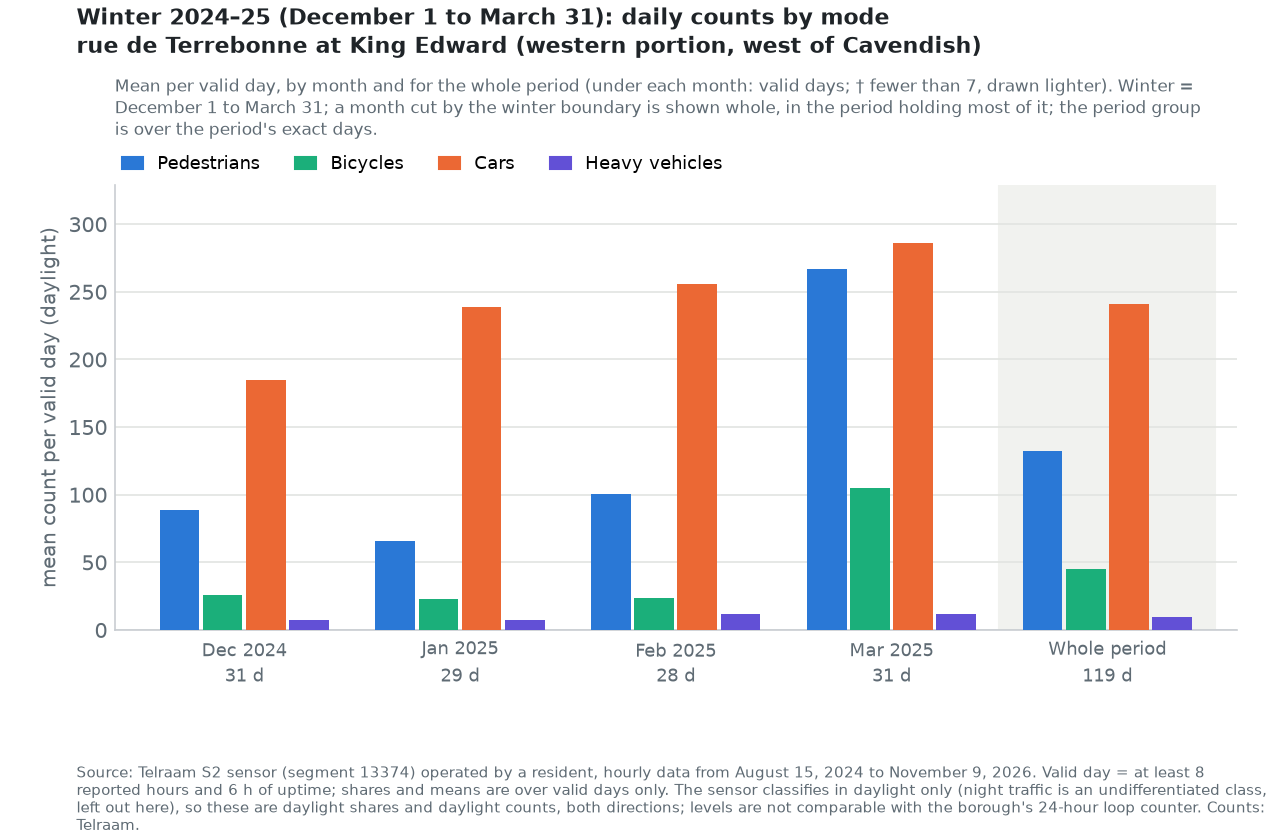
\includegraphics[width=0.86\textwidth]{../figures/mode-shares/dec1/counts_west_winter-2024-25.png}\end{frame}
\begin{frame}{Draper (eastern portion), non--winter 2024: who used the street}\centering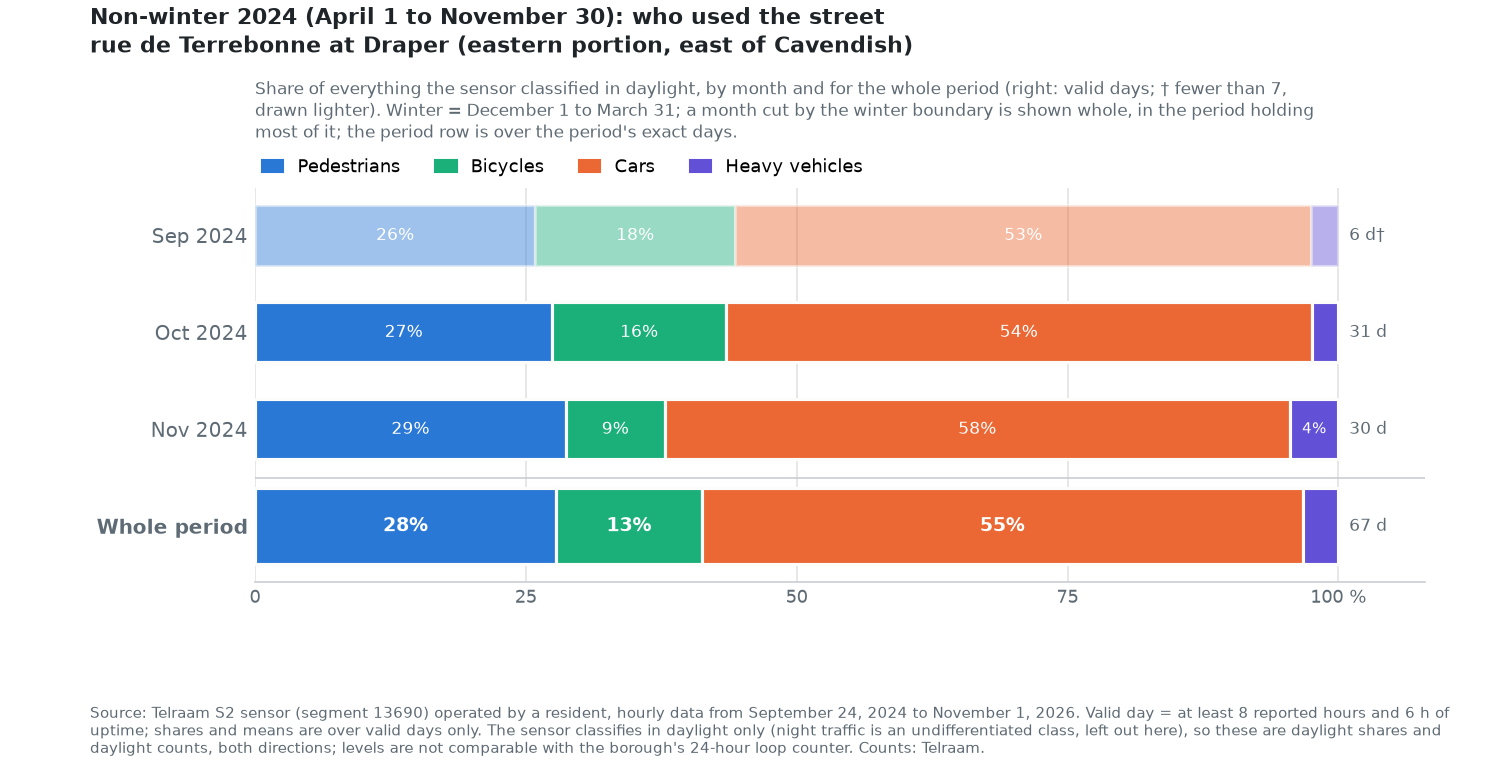
\includegraphics[width=0.8\textwidth]{../figures/mode-shares/dec1/shares_east_non-winter-2024.png}\end{frame}
\begin{frame}{Draper (eastern portion), non--winter 2026: who used the street}\centering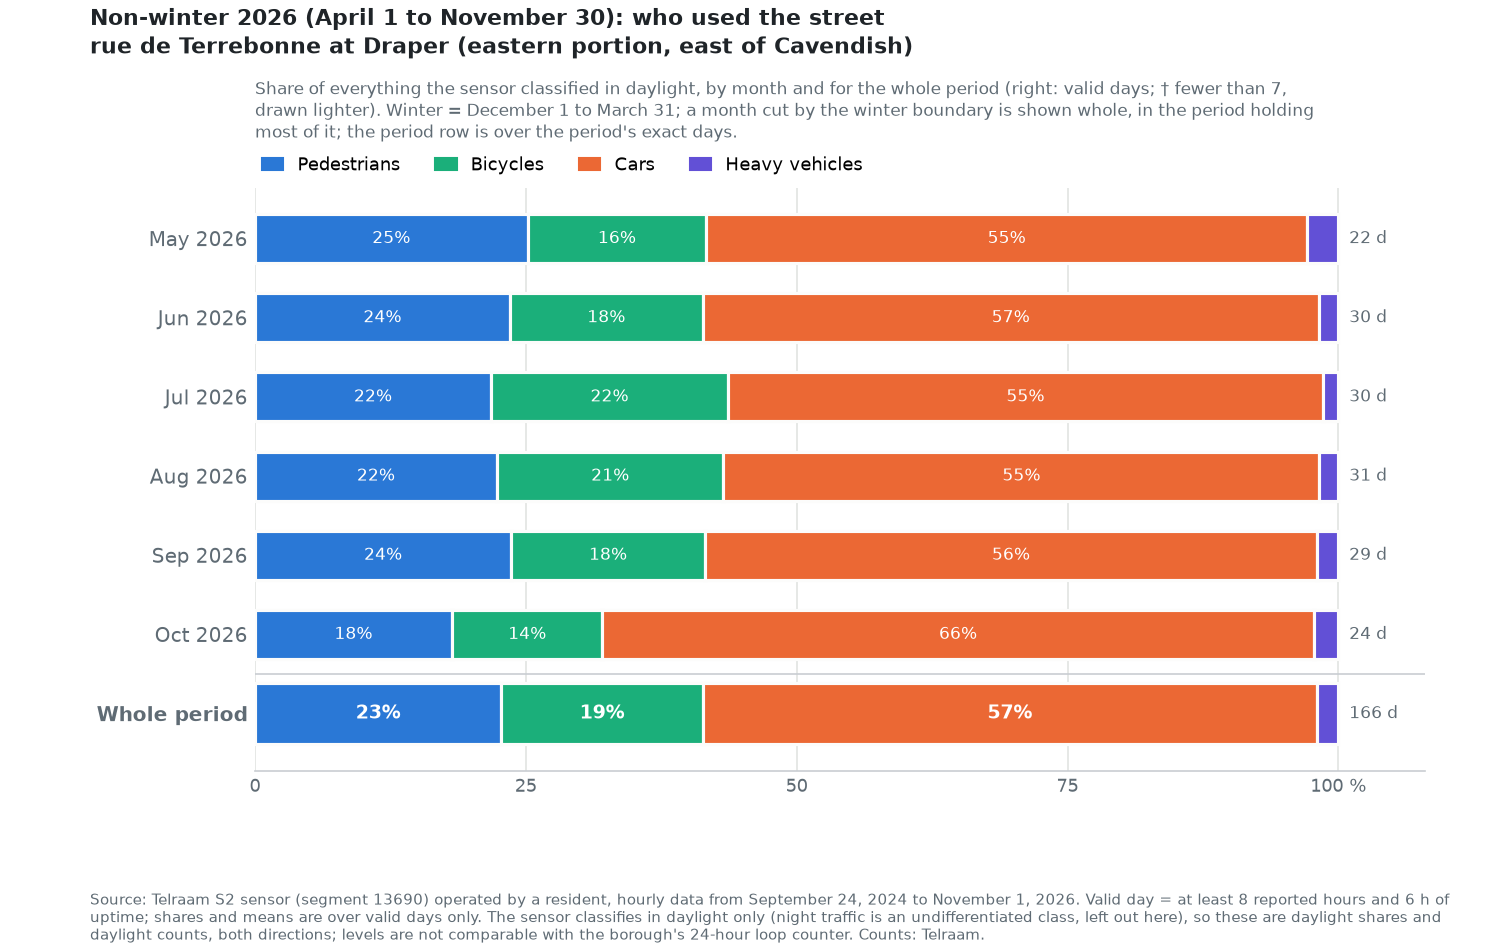
\includegraphics[width=0.8\textwidth]{../figures/mode-shares/dec1/shares_east_non-winter-2026.png}\end{frame}
\begin{frame}{Draper (eastern portion), winter 2025--26: who used the street}\centering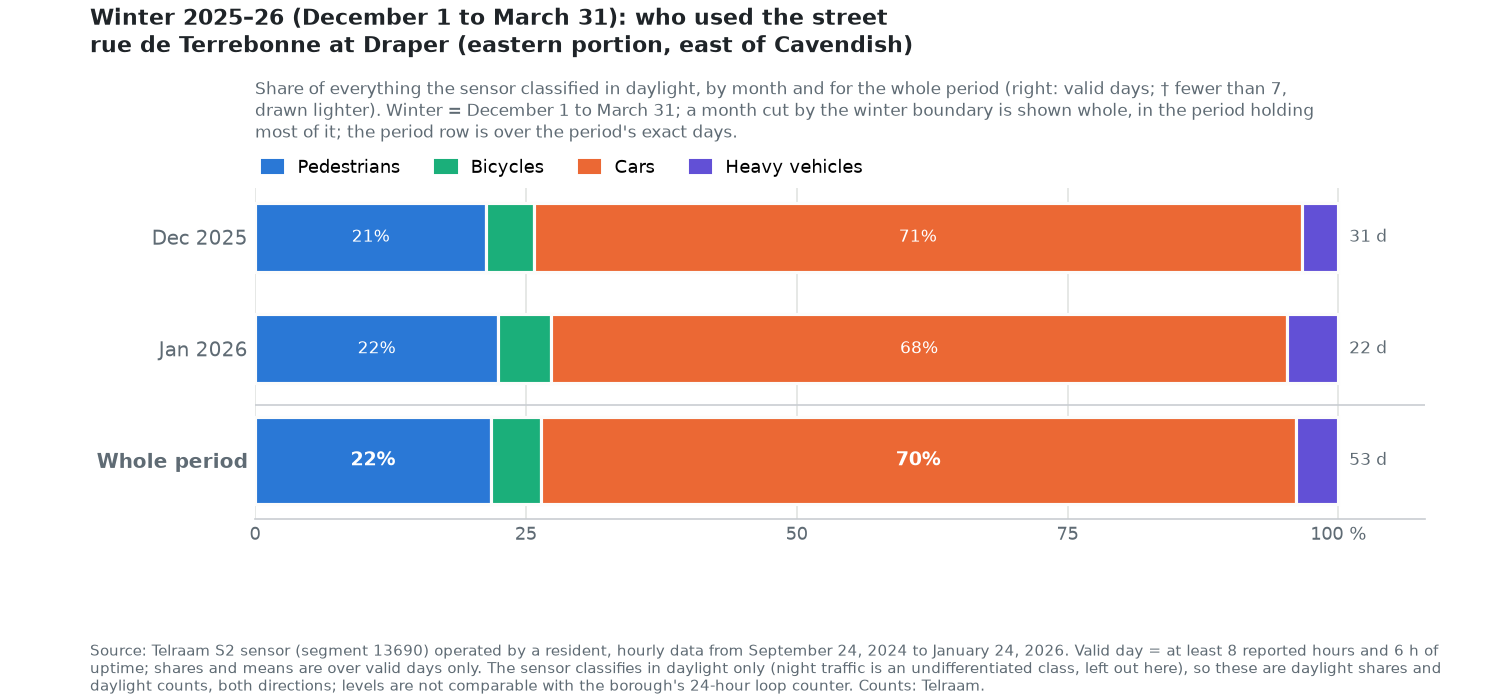
\includegraphics[width=0.8\textwidth]{../figures/mode-shares/dec1/shares_east_winter-2025-26.png}\end{frame}
\begin{frame}{Kensington loop (24 h), non--winter 2026: who used the street}\centering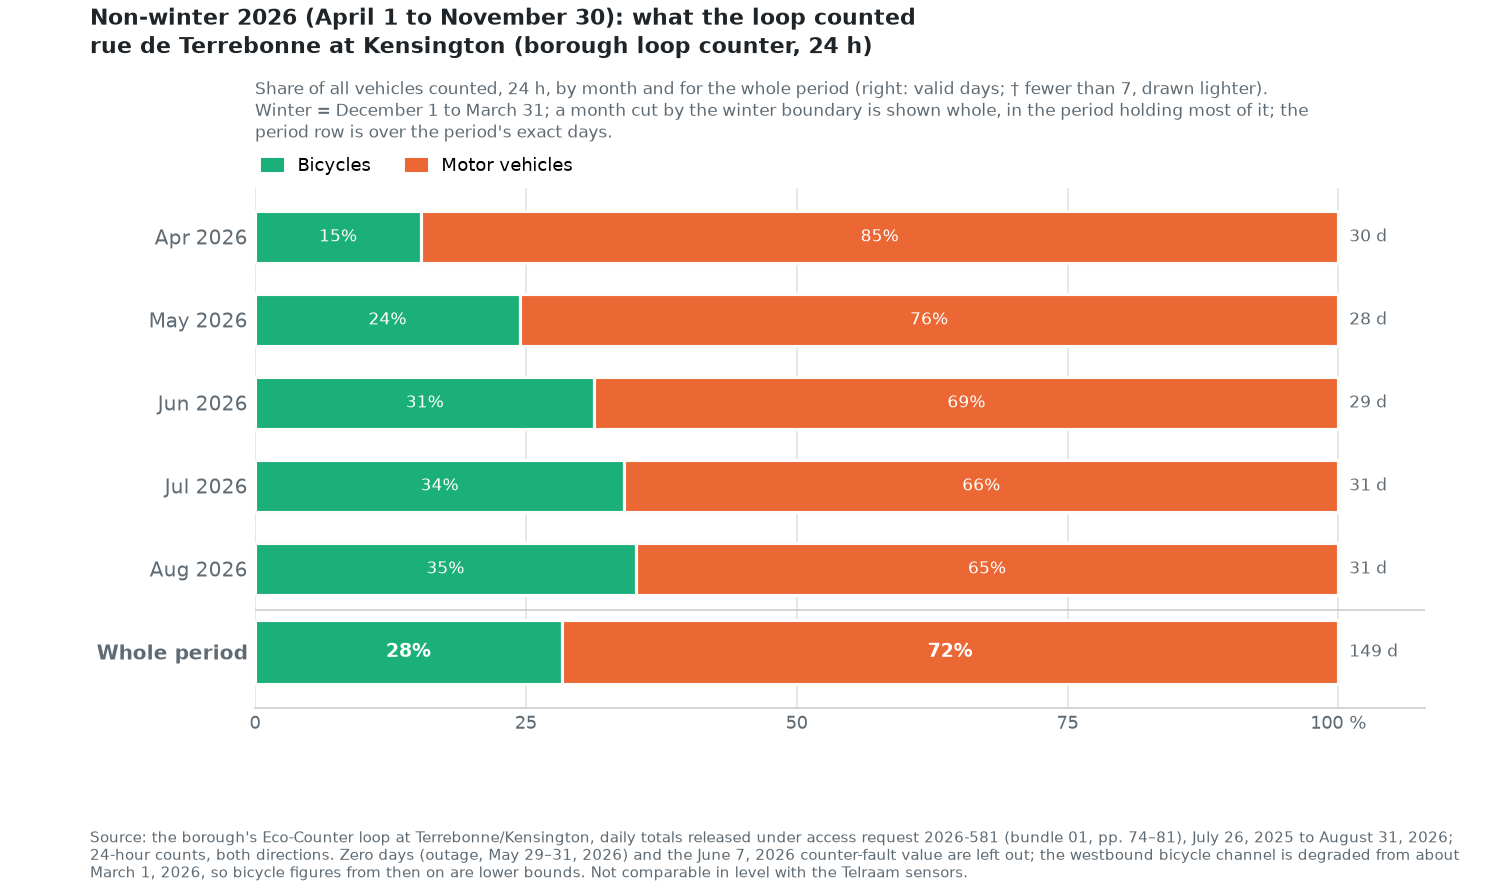
\includegraphics[width=0.8\textwidth]{../figures/mode-shares/dec1/shares_kensington_non-winter-2026.png}\end{frame}
\begin{frame}{King Edward (western portion), non--winter 2024: who used the street}\centering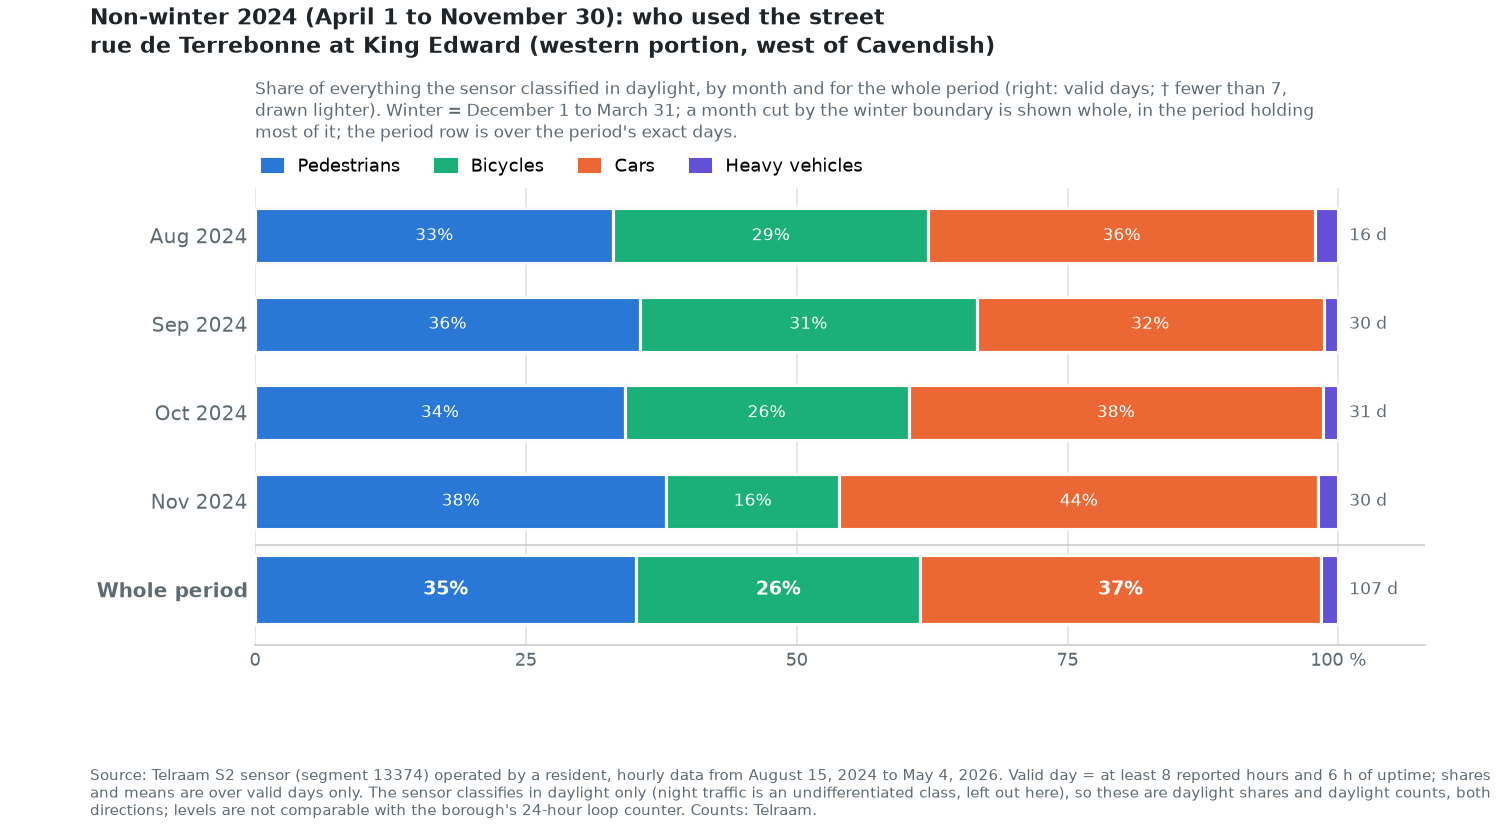
\includegraphics[width=0.8\textwidth]{../figures/mode-shares/dec1/shares_west_non-winter-2024.png}\end{frame}
\begin{frame}{King Edward (western portion), non--winter 2026: who used the street}\centering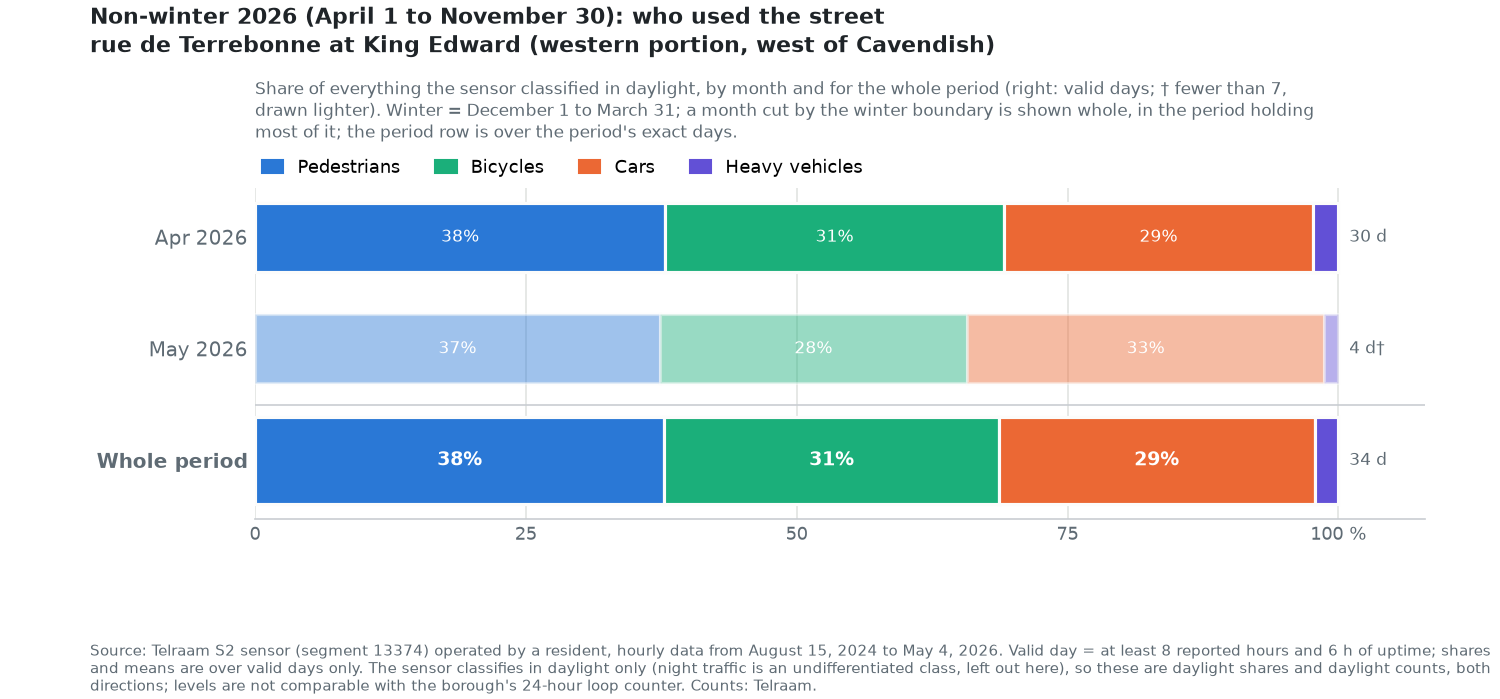
\includegraphics[width=0.8\textwidth]{../figures/mode-shares/dec1/shares_west_non-winter-2026.png}\end{frame}
\begin{frame}{Draper (eastern portion): same months, year over year}\centering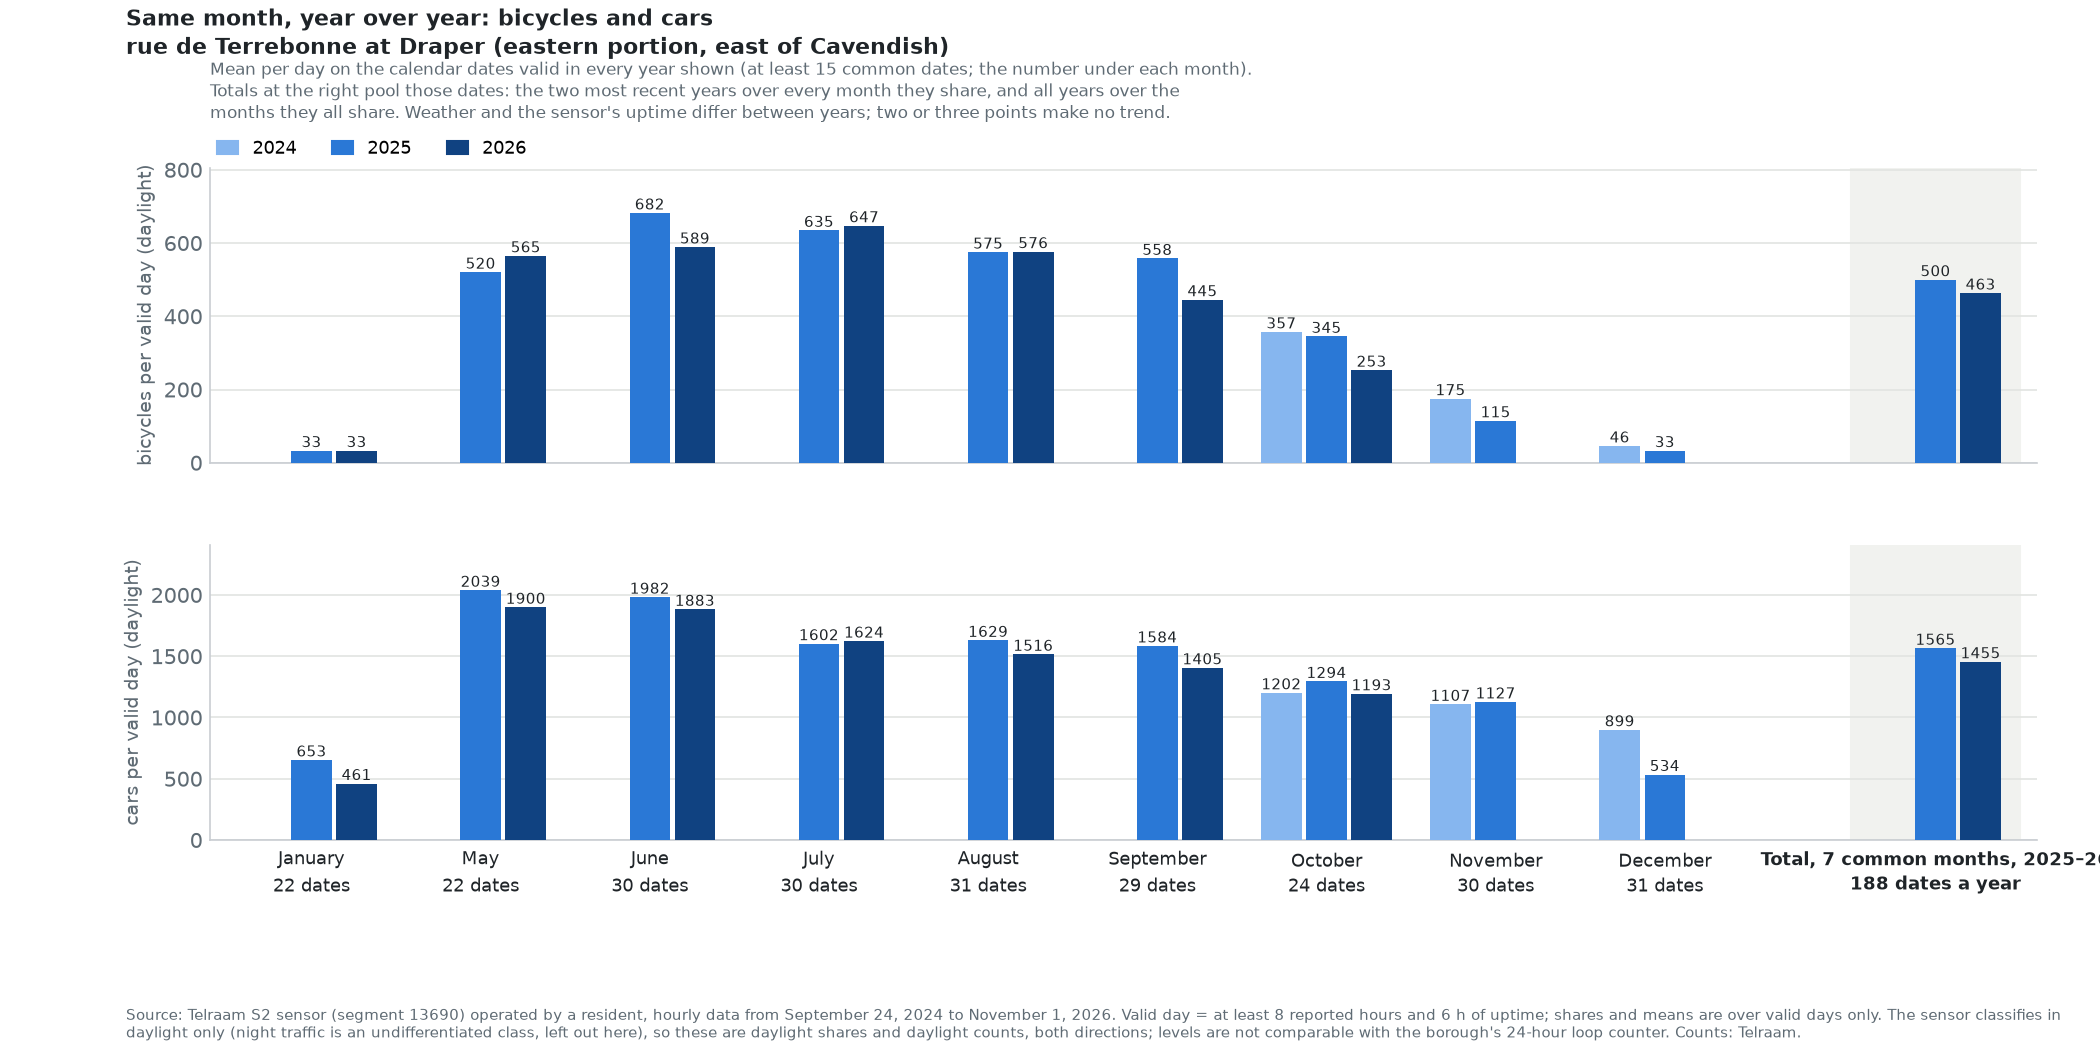
\includegraphics[width=0.86\textwidth]{../figures/mode-shares/dec1/yoy_east.png}\end{frame}
\begin{frame}{Kensington loop (24 h): same months, year over year}\centering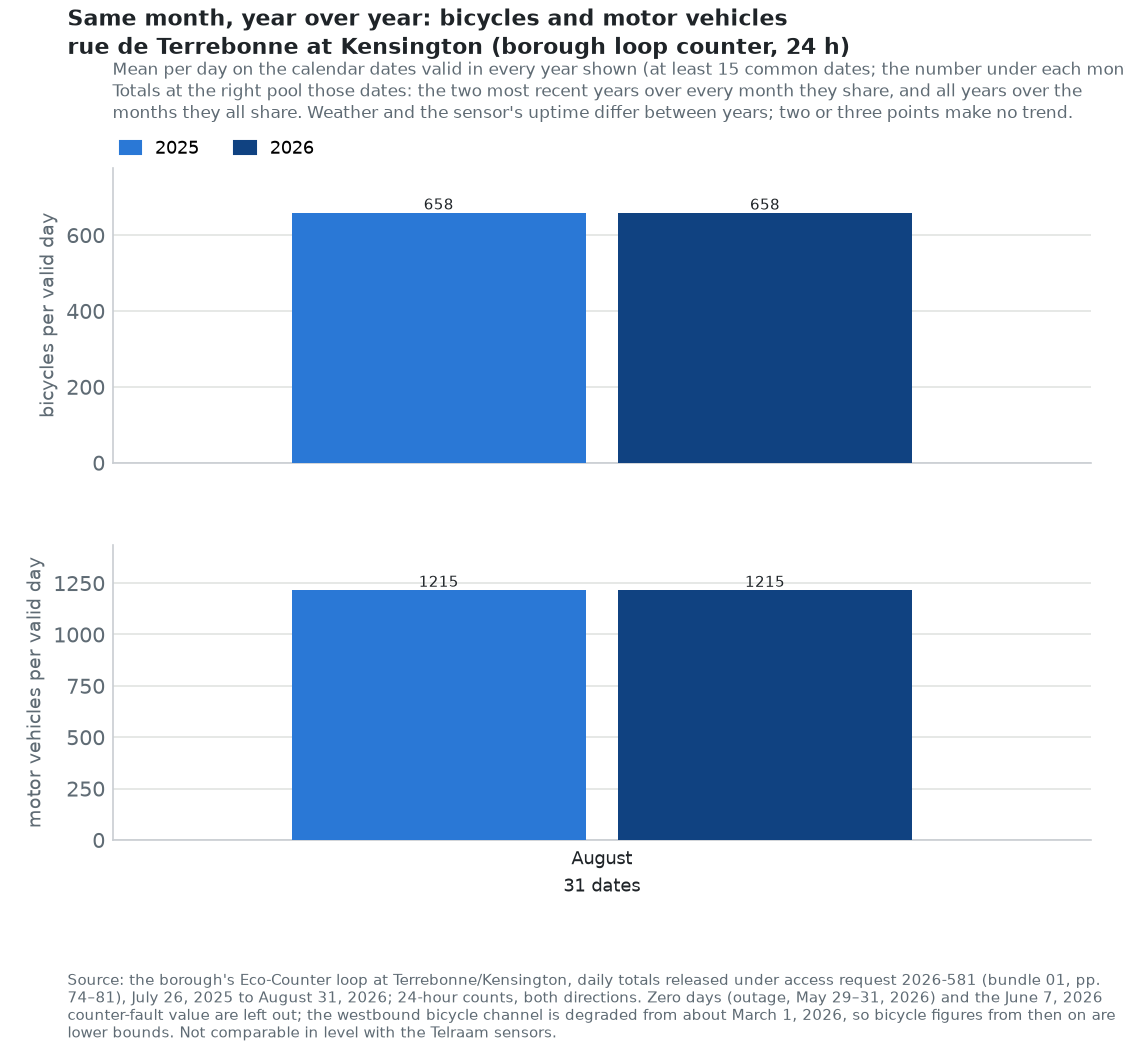
\includegraphics[width=0.86\textwidth]{../figures/mode-shares/dec1/yoy_kensington.png}\end{frame}
\end{document}
